\input{setup.tex}

% Режим шаблона (должен быть включен один из трех)
%\ВКРtrue
\Практикаtrue
%\Курсоваяtrue

\newcommand{\Дисциплина}{<<Методы и алгоритмы обработки изображений>>} % для курсовой
\newcommand{\КодСпециальности}{09.03.04} % Курсовая
\newcommand{\Специальность}{Программная инженерия} % Курсовая
\newcommand{\Тема}{} % ВКР Курсовая
\newcommand{\ГдеПроводитсяПрактика}{ООО «Предприятие ВТИ-Сервис»} % для практики
\newcommand{\РуководительПрактПредпр}{} % для практики
\newcommand{\ДолжнРуководительПрактПредпр}{} % для практики
\newcommand{\РуководительПрактУнивер}{Чаплыгин А. А.} % для практики
\newcommand{\ДолжнРуководительПрактУнивер}{к.т.н. доцент} % для практики
\newcommand{\Автор}{И.С. Глазунов}
\newcommand{\АвторРод}{Петров М.Е.}
\newcommand{\АвторПолностьюРод}{Петрова Михаила Евгеньевича} % для практики
\newcommand{\Шифр}{22-06-0214}
\newcommand{\Курс}{4} % для практики
\newcommand{\Группа}{ПО-22б}
\newcommand{\Руководитель}{Р. А. Томакова} % для ВКР и курсовой
\newcommand{\Нормоконтроль}{А. А. Чаплыгин} % для ВКР
\newcommand{\ЗавКаф}{А. В. Малышев} % для ВКР
\newcommand{\ДатаПриказа}{«07» апреля 2023~г.} % для ВКР
\newcommand{\НомерПриказа}{1505-с} % для ВКР
\newcommand{\СрокПредоставления}{} % для ВКР, курсового

\begin{document}
\maketitle
\ifПрактика{}\else{
   \newpage
\begin{center}
\large\textbf{Минобрнауки России}

\large\textbf{Юго-Западный государственный университет}
\vskip 1em
\normalsize{Кафедра программной инженерии}
\vskip 1em
\ifВКР{
        \begin{flushright}
        \begin{tabular}{p{.4\textwidth}}
        \centrow УТВЕРЖДАЮ: \\
        \centrow Заведующий кафедрой \\
        \hrulefill \\
        \setarstrut{\footnotesize}
        \centrow\footnotesize{(подпись, инициалы, фамилия)}\\
        \restorearstrut
        «\underline{\hspace{1cm}}»
        \underline{\hspace{3cm}}
        20\underline{\hspace{1cm}} г.\\
        \end{tabular}
        \end{flushright}
        }\fi
\end{center}
\vspace{1em}
  \begin{center}
  \large
\ifВКР{
ЗАДАНИЕ НА ВЫПУСКНУЮ КВАЛИФИКАЦИОННУЮ РАБОТУ
  ПО ПРОГРАММЕ БАКАЛАВРИАТА}
  \else
ЗАДАНИЕ НА КУРСОВУЮ РАБОТУ (ПРОЕКТ)
\fi
\normalsize
  \end{center}
\vspace{1em}
{\parindent0pt
  Студента \АвторРод, шифр\ \Шифр, группа \Группа
  
1. Тема «\Тема\ \ТемаВтораяСтрока»
\ifВКР{
	утверждена приказом ректора ЮЗГУ от \ДатаПриказа\ № \НомерПриказа
}\fi.

2. Срок предоставления работы к защите \СрокПредоставления

3. Исходные данные для создания программной системы:

3.1. Перечень решаемых задач:}

\renewcommand\labelenumi{\theenumi)}

\begin{enumerate}
\item Провести анализ деятельности редакционно-издательского отдела вуза и выявить проблематику традиционного подхода к проверке учебно-методических материалов;
\item Разработать концептуальную модель информационно-аналитической системы;
\item Спроектировать архитектуру системы, включая базу данных и веб-интерфейс;
\item Реализовать систему средствами веб-технологий (Python, FastAPI, PostgreSQL, HTML, CSS, JavaScript);
\item Разработать модуль автоматической проверки оформления документов формата DOCX (шрифт, отступы, интервалы, нумерация страниц);
\item Разработать модуль генерации титульных листов для методических указаний, учебных пособий и монографий.
\end{enumerate}

{\parindent0pt

3.2. Входные данные и требуемые результаты для программы:}
\begin{enumerate}
\item Входными данными для программной системы являются: файлы формата DOCX (методические указания, учебные пособия, монографии), параметры для генерации титульных листов (название, автор, рецензенты, УДК, ISBN, описание), учётные данные пользователей (ФИО, email, пароль, факультет, кафедра, роль).

\item Выходными данными являются: результаты автоматической проверки документа (список ошибок с указанием страниц), исправленный документ с визуально выделенными ошибками, PDF-отчёт о проверке, сгенерированный титульный лист в формате DOCX, статистические отчёты по загруженным документам, JWT-токены для авторизации, подтверждение отправки файлов на электронную почту РИО.
\end{enumerate}

{\parindent0pt

4. Содержание работы (по разделам):

4.1. Введение.

4.2. Анализ предметной области.

4.3. Техническое задание: основание для разработки, назначение разработки,
требования к программной системе, требования к оформлению документации.

4.4. Технический проект: общие сведения о программной системе, проект
данных программной системы (ER-модель, реляционная модель), проектирование архитектуры программной системы, проектирование пользовательского интерфейса программной системы.

4.5. Рабочий проект: маршруты приложения, спецификация контроллеров, системное тестирование разработанного веб-сайта.

4.6. Заключение.

4.7. Список использованных источников.

5. Перечень графического материала:

\списокПлакатов

\vskip 2em
\begin{tabular}{p{6.8cm}C{3.8cm}C{4.8cm}}
	Руководитель \ifВКР{ВКР}\else работы (проекта) \fi & \lhrulefill{\fill} & \fillcenter\Руководитель\\
	\setarstrut{\footnotesize}
	& \footnotesize{(подпись, дата)} & \footnotesize{(инициалы, фамилия)}\\
	\restorearstrut
	Задание принял к исполнению & \lhrulefill{\fill} & \fillcenter\Автор\\
	\setarstrut{\footnotesize}
	& \footnotesize{(подпись, дата)} & \footnotesize{(инициалы, фамилия)}\\
	\restorearstrut
\end{tabular}
}

\renewcommand\labelenumi{\theenumi.}

   \abstract{РЕФЕРАТ}

Объем работы равен \formbytotal{lastpage}{страниц}{е}{ам}{ам}. Работа содержит \formbytotal{figurecnt}{иллюстраци}{ю}{и}{й}, \formbytotal{tablecnt}{таблиц}{у}{ы}{} 
и \arabic{bibcount} библиографических источников. Количество приложений – 2. Графический материал представлен в приложении А. Фрагменты исходного кода представлены в приложении Б.

Перечень ключевых слов: Python, REST API, FastAPI, PostgreSQL,
информационно-аналитическая система, проверка учебно-методических материалов, веб-приложение, генерация титульных листов, PDF-отчёты.

Объектом разработки является информационно-аналитическая система автоматизации проверки и обработки учебно-методических материалов редакционно-издательского отдела.

Целью работы является разработка информационно-аналитической системы для автоматизации процессов проверки, оформления и сопровождения учебно-методических документов.

Разработанная система реализована на языке Python с использованием web-фреймворка FastAPI и СУБД PostgreSQL. Клиентская часть разработана с применением HTML, CSS и JavaScript. Взаимодействие между компонентами системы осуществляется через REST API.

Архитектура системы построена по клиент-серверной модели. Серверная часть выполняет обработку запросов пользователей, проверку DOCX-документов, генерацию титульных листов, формирование PDF-отчётов и взаимодействие с базой данных. Клиентская часть предоставляет web-интерфейс для загрузки документов и просмотра результатов проверки.

В системе реализован модуль автоматической проверки DOCX-документов, выполняющий анализ параметров форматирования и структуры учебно-методических материалов. Результаты проверки используются для формирования PDF-отчётов с перечнем найденных ошибок..

Разработанная система позволяет сократить время проверки документов, уменьшить количество ошибок оформления и повысить эффективность работы редакционно-издательского отдела.



\selectlanguage{english}
\abstract{ABSTRACT}

The volume of work is \formbytotal{lastpage}{page}{}{s}{s}. The work contains \formbytotal{figurecnt}{illustration}{}{s}{s},\formbytotal{tablecnt}{tables}{}{s}{s} and \arabic{bibcount} bibliographic sources. The number of applications is 2. The graphic material is presented in Appendix A. Fragments of the source code are presented in Appendix B.

List of keywords: Python, REST API, FastAPI, PostgreSQL,
information and analytical system, verification of teaching materials, web application, generation of cover pages, PDF reports.

The object of the development is an information and analytical automation system for checking and processing educational and methodological materials of the editorial and publishing department.

The purpose of the work is to develop an information and analytical system for automating the processes of verification, registration and maintenance of educational and methodological documents.

The developed system is implemented in Python using the FastAPI web framework and the PostgreSQL database management system. The client side is developed using HTML, CSS, and JavaScript. The interaction between the system components is carried out through the REST API.

The architecture of the system is based on the client-server model. The server side processes user requests, validates DOCX documents, generates title pages, generates PDF reports, and interacts with the database. The client side provides a web interface for downloading documents and viewing the verification results.

The system implements an automatic verification module for DOCX documents, which analyzes the formatting parameters and structure of teaching materials. The verification results are used to generate PDF reports with a list of errors found..

The developed system makes it possible to reduce the time needed to check documents, reduce the number of design errors, and improve the efficiency of the editorial and publishing department.
\selectlanguage{russian}}\fi
\tableofcontents
\section*{ОБОЗНАЧЕНИЯ И СОКРАЩЕНИЯ}

РИО~--- редакционно-издательский отдел.

СУБД~--- система управления базами данных.

ТЗ~--- техническое задание.

ТП~--- технический проект.

ФИО~--- фамилия, имя, отчество.

API (Application Programming Interface)~--- программный интерфейс приложения.

CSS (Cascading Style Sheets)~--- каскадные таблицы стилей.

DOCX~--- формат файлов текстового редактора Microsoft Word, основанный на Office Open XML.

HTML (HyperText Markup Language)~--- язык разметки гипертекста.

HTTP (HyperText Transfer Protocol)~--- протокол передачи гипертекста.

HTTPS (HyperText Transfer Protocol Secure)~--- защищённый протокол передачи гипертекста.

JSON (JavaScript Object Notation)~--- текстовый формат обмена данными на основе синтаксиса JavaScript.

PDF (Portable Document Format)~--- переносимый формат документов.

REST (Representational State Transfer)~--- архитектурный стиль взаимодействия компонентов распределённой системы.

SPA (Single Page Application)~--- одностраничное веб-приложение.

SQL (Structured Query Language)~--- язык структурированных запросов.

XSS (Cross-Site Scripting)~--- межсайтовый скриптинг.
\ifПрактика{}\else{\section*{ВВЕДЕНИЕ}
\addcontentsline{toc}{section}{ВВЕДЕНИЕ}

В условиях стремительного роста объёмов цифровой информации особую роль приобретают методы эффективного хранения и передачи мультимедийных данных. Значительную часть таких данных составляют цифровые изображения, которые широко используются в информационных системах, веб-приложениях, мобильных устройствах и средствах передачи данных. При этом исходные изображения обладают большим объёмом, что создаёт дополнительные требования к пропускной способности каналов связи и объёму памяти.

Одним из наиболее распространённых способов уменьшения объёма графических данных является сжатие изображений с потерями, позволяющее существенно сократить размер файла при сохранении приемлемого визуального качества. Наибольшее распространение получил стандарт JPEG, основанный на использовании дискретного косинусного преобразования, квантования и субдискретизации цветовых компонент. Данный стандарт применяется в большинстве цифровых камер, графических редакторов и веб-браузеров, что делает его изучение и практическую реализацию актуальной задачей.

В рамках данной курсовой работы рассматривается процесс программной реализации алгоритма JPEG-сжатия растровых изображений. Особое внимание уделяется поэтапной реализации ключевых компонентов алгоритма, включая преобразование цветового пространства RGB в YCbCr, хроматическую субдискретизацию формата 4:2:0, дискретное косинусное преобразование, квантование коэффициентов и последующее восстановление изображения для оценки визуального качества.

Целью данной курсовой работы является разработка программного средства для сжатия изображений в формате JPEG с возможностью управления параметром качества и визуального анализа результатов сжатия.

Для достижения поставленной цели необходимо решить следующие задачи:
\begin{itemize}
	\item изучить принципы и этапы алгоритма JPEG-сжатия изображений;
	\item реализовать преобразование цветового пространства RGB в YCbCr и обратно;
	\item реализовать дискретное косинусное преобразование и обратное преобразование;
	\item разработать механизм квантования с учётом параметра качества;
	\item реализовать хроматическую субдискретизацию и апсемплинг;
	\item разработать графический интерфейс для взаимодействия с пользователем;
	\item провести тестирование программы и анализ полученных результатов.
\end{itemize}
}\fi
\section{Анализ предметной области}

\subsection{Характеристика деятельности редакционно-издательского отдела вуза}

Редакционно-издательский отдел (РИО) высшего учебного заведения является структурным подразделением, обеспечивающим подготовку, проверку, оформление и выпуск учебно-методической, научной и справочной литературы, используемой в образовательном процессе. К числу основных материалов, поступающих в РИО, относятся методические указания, учебные пособия, практикумы, монографии, сборники научных трудов и иные издания.

Современный образовательный процесс требует постоянного обновления учебно-методической базы. Изменение федеральных государственных образовательных стандартов, развитие научных направлений, внедрение новых технологий обучения и цифровых платформ обуславливают регулярную подготовку новых материалов преподавателями университета.

РИО выполняет функции организационного и нормативного сопровождения издательской деятельности вуза. Сотрудники подразделения принимают материалы от авторов, проверяют их соответствие установленным требованиям оформления, контролируют наличие обязательных структурных элементов, подготавливают замечания, формируют титульные листы, а также ведут учёт поступивших и утверждённых работ.

В условиях большого количества авторов и поступающих документов особую значимость приобретают скорость обработки материалов, точность проверки и удобство взаимодействия между преподавателями и сотрудниками отдела. Эффективность деятельности РИО напрямую влияет на своевременное обеспечение образовательного процесса актуальными учебными материалами.

\subsection{Проблематика традиционного подхода к организации проверки материалов}

Традиционный подход к работе редакционно-издательского отдела, основанный на ручной обработке документов, сопровождается рядом существенных недостатков, снижающих эффективность работы подразделения:
\begin{enumerate}
\item{Высокая трудоёмкость проверки оформления.} В большинстве случаев сотрудники РИО вручную проверяют поступившие документы на соответствие установленным требованиям: параметры шрифта, интервалы, отступы, структура заголовков, оформление списков литературы, таблиц, рисунков и других элементов. При большом количестве работ такой процесс занимает значительное время.

\item{Высокая вероятность человеческих ошибок.} Ручная проверка не гарантирует обнаружение всех нарушений оформления. Из-за большого объёма текста, однотипности операций и человеческого фактора часть ошибок может остаться незамеченной, что приводит к возврату материалов на доработку уже на поздних этапах.

\item{Длительное взаимодействие с авторами.} После выявления замечаний сотрудник вынужден вручную составлять перечень ошибок либо вносить исправления в режиме рецензирования документа. Это увеличивает сроки согласования и повторной подачи материалов.

\item{Отсутствие централизованного хранилища работ.} Готовые и поступившие материалы часто хранятся в отдельных папках, на персональных компьютерах или сетевых дисках. Это затрудняет поиск ранее утверждённых изданий, ведение архива и получение статистических сведений.

\item{Сложность формирования отчётности.} Для подготовки отчётов по количеству проверенных работ, числу авторов, срокам обработки и видам материалов требуется вручную собирать данные из различных источников. Это увеличивает нагрузку на сотрудников и снижает оперативность получения информации.

\item{Отсутствие унифицированных шаблонов.} Авторы нередко подготавливают титульные листы и иные элементы документа самостоятельно, что приводит к многочисленным отклонениям от утверждённых образцов и повторным исправлениям.
\end{enumerate}

Таким образом, ручной подход к организации работы РИО не обеспечивает необходимой скорости, точности и удобства обработки документов в современных условиях.

\subsection{Обоснование необходимости автоматизации}

Решение перечисленных проблем возможно путём внедрения специализированной информационно-аналитической системы для автоматизации деятельности редакционно-издательского отдела вуза.

Разрабатываемая система должна обеспечить:

\begin{itemize}
	\item загрузку пользователями учебно-методических и научных материалов через веб-интерфейс;
	\item автоматическую проверку документов на соответствие требованиям оформления;
	\item формирование подробного отчёта с перечнем найденных ошибок;
	\item автоматическое создание файла формата DOCX с выделенными нарушениями;
	\item автоматическое сохранение корректно оформленных работ в централизованном хранилище;
	\item ведение статистики поступивших, проверенных и утверждённых материалов;
	\item генерацию титульных листов по утверждённым шаблонам;
	\item разграничение прав доступа между авторами, редакторами и администраторами системы;
	\item удобный интерфейс взаимодействия пользователей с системой.
\end{itemize}

Автоматизация позволит существенно сократить время проверки материалов, снизить количество ошибок, ускорить процесс согласования документов и обеспечить прозрачный контроль деятельности подразделения.

\subsection{Анализ существующих систем автоматизации документооборота и проверки документов}

На современном рынке представлены различные программные решения, связанные с управлением документами, совместной работой и проверкой текстовых материалов. Однако большинство из них не ориентировано на специфику работы редакционно-издательского отдела вуза.

\subsubsection{Microsoft Word и встроенные средства рецензирования}

Текстовый редактор Microsoft Word широко применяется для подготовки и проверки документов. Он предоставляет следующие возможности:

\begin{itemize}
	\item создание и редактирование документов;
	\item проверка орфографии и грамматики;
	\item режим рецензирования и внесения исправлений;
	\item использование шаблонов оформления.
\end{itemize}

Недостатком данного подхода является отсутствие автоматизированной проверки документа на соответствие локальным требованиям конкретного вуза. Проверка структуры, параметров оформления и соответствия внутренним стандартам выполняется вручную.

\subsubsection{Google Docs}

Google Docs является облачным сервисом для совместной работы с документами. Его возможности включают:

\begin{itemize}
	\item онлайн-редактирование файлов;
	\item совместную работу нескольких пользователей;
	\item систему комментариев и предложений;
	\item хранение документов в облаке.
\end{itemize}

Несмотря на удобство совместного редактирования, сервис не предоставляет специализированных механизмов автоматической проверки учебно-методических материалов по требованиям университета, а также не содержит функций аналитической отчётности для РИО.

\subsubsection{Системы электронного документооборота}

Корпоративные системы электронного документооборота предназначены для регистрации, маршрутизации и хранения документов. Они позволяют:

\begin{itemize}
	\item вести архив документов;
	\item организовывать согласование файлов;
	\item разграничивать права доступа;
	\item контролировать исполнение задач.
\end{itemize}

Однако подобные системы являются универсальными решениями и не включают инструменты интеллектуального анализа оформления документов DOCX, автоматического подчёркивания ошибок и генерации титульных листов.

\subsubsection{Вывод по анализу аналогов}

Проведённый анализ существующих решений показал, что универсальные офисные продукты и системы электронного документооборота способны решать лишь отдельные задачи редакционно-издательского отдела.

Одни системы обеспечивают редактирование документов, другие --- хранение файлов и организацию согласования, однако ни одно из рассмотренных решений не сочетает в себе функции автоматической проверки оформления методических материалов, генерации отчётов об ошибках, формирования исправленного DOCX-файла и накопления статистики работы подразделения.

Следовательно, наиболее целесообразным является создание собственной специализированной информационно-аналитической системы, учитывающей особенности документооборота и нормативные требования конкретного высшего учебного заведения.

\subsection{Постановка задач на разработку}

На основании проведённого анализа были сформулированы следующие задачи, которые должна решать разрабатываемая система:

\begin{enumerate}
	\item Обеспечить регистрацию и авторизацию пользователей с разграничением прав доступа.
	\item Реализовать загрузку методических, учебных и научных материалов в формате DOCX.
	\item Выполнить автоматическую проверку документов на соответствие установленным требованиям оформления.
	\item Формировать отчёт с перечнем найденных нарушений.
	\item Создавать копию документа DOCX с визуальным выделением ошибок.
	\item Автоматически сохранять корректно оформленные работы в централизованной базе данных.
	\item Реализовать хранение и поиск ранее загруженных материалов.
	\item Предоставить средства формирования статистической и аналитической отчётности.
	\item Реализовать модуль автоматического создания титульных листов по шаблону вуза.
	\item Создать удобный веб-интерфейс для пользователей и административную панель для управления системой.
\end{enumerate}
\section{Техническое задание}

\subsection{Основание для разработки}

Основанием для разработки является задание на выпускную квалификационную работу бакалавра "Информационно-аналитическая система для РИО вуза.Разработка сервиса "Методические указания"

\subsection{Цель и назначение разработки}

Основной целью работы является разработка и внедрение информационно-аналитической системы для автоматизации процессов проверки, хранения и сопровождения учебно-методических и научных материалов, поступающих в редакционно-издательский отдел вуза.

Информационно-аналитическая система предназначена для преподавателей, являющизся авторами учебно-методических разработок и сотрудников релакционно-издательского вуза.

\subsection{Требования к функциональности}

Информационная система должна обеспечивать выполнение следующих функций:

\begin{enumerate}
	\item {Управление пользователями.} Система должна обеспечивать регистрацию и авторизацию пользователей по логину и паролю. Должно быть реализовано разграничение прав доступа: администратор, редактор, пользователь. Администратор должен иметь возможность управления учётными записями пользователей.
	
	\item {Загрузка документов.} Пользователь должен иметь возможность загружать методические материалы, учебные пособия, монографии и иные документы в формате DOCX через веб-интерфейс системы.
	
	\item {Автоматическая проверка оформления.} После загрузки документа система должна автоматически анализировать файл на соответствие установленным требованиям оформления. Проверка должна включать контроль структуры документа, параметров шрифта, интервалов, отступов, заголовков, таблиц, изображений, списков литературы и иных элементов.
	
	\item {Формирование отчёта об ошибках.} По завершении анализа система должна формировать отчёт, содержащий перечень обнаруженных нарушений, описание ошибок и рекомендации по их устранению.
	
	\item {Создание документа с выделением ошибок.} Система должна создавать копию загруженного документа в формате DOCX, в которой найденные ошибки визуально выделены средствами форматирования.
	
	\item {Хранение корректных документов.} Если загруженный документ соответствует всем требованиям, он должен автоматически сохраняться в централизованной базе данных или файловом архиве системы.
	
	\item {Поиск и просмотр документов.} Система должна обеспечивать просмотр списка ранее загруженных материалов, поиск по названию, автору, дате загрузки, статусу проверки и другим параметрам.
	
	\item {Генерация титульных листов.} Пользователь должен иметь возможность заполнить форму с исходными данными, после чего система должна автоматически сформировать титульный лист по утверждённому шаблону вуза.
	
	\item {Статистика и аналитика.} Система должна формировать сводные данные по количеству загруженных документов, числу успешных проверок, количеству найденных ошибок, активности пользователей и временным показателям обработки материалов.
	
	\item {Логирование действий.} Система должна сохранять сведения о действиях пользователей: загрузка файлов, проверка документов, вход в систему, генерация титульных листов и иные операции.
\end{enumerate}

\subsection{Требования к интерфейсу}

Интерфейс информационной системы представляет собой веб-приложение с единым современным стилем оформления, обеспечивающее удобную и интуитивно понятную навигацию. Пользовательский интерфейс должен быть адаптирован для работы в распространённых браузерах и обеспечивать быстрый доступ к основным функциям системы.

Основные элементы интерфейса включают:

\begin{itemize}
	\item главную страницу системы;
	\item форму авторизации и регистрации пользователей;
	\item личный кабинет пользователя;
	\item страницу загрузки документов на проверку;
	\item страницу просмотра результатов проверки;
	\item страницу архива сохранённых документов;
	\item страницу генерации титульных листов;
	\item административную панель управления пользователями;
	\item модуль просмотра статистики и аналитических данных.
\end{itemize}

На рисунке~\ref{fig:authorization} представлена страница авторизации системы.

\begin{figure}[h]
	\centering
	
\includegraphics[width=1\textwidth]{authorization.png}
	\caption{Страница авторизации}
	\label{fig:authorization}
\end{figure}

Как показано на рисунке, форма авторизации содержит поля ввода логина и пароля, кнопку входа в систему, а также элементы перехода к регистрации нового пользователя. После успешной авторизации пользователь получает доступ к функциональным возможностям системы в соответствии со своей ролью.

На рисунке~\ref{fig:profile} представлен внешний вид личного кабинета пользователя.

\begin{figure}[h]
	\centering
	
\includegraphics[width=1\textwidth]{profile.png}
	\caption{Личный кабинет пользователя}
	\label{fig:profile}
\end{figure}

Личный кабинет содержит навигационное меню, сведения о текущем пользователе, основные разделы системы, а также быстрый доступ к загрузке документов, архиву файлов и генерации титульных листов.

\clearpage
На рисунке~\ref{fig:filecheck} представлена страница проверки документов.

\begin{figure}[h]
	\centering
	
\includegraphics[width=1\textwidth]{filecheck.png}
	\caption{Страница проверки документов}
	\label{fig:filecheck}
\end{figure}

Данная страница содержит форму выбора файла формата DOCX, кнопку запуска автоматической проверки, область отображения текущего статуса обработки и результаты анализа после завершения проверки.

На рисунке~\ref{fig:titlegen} представлена страница генерации титульных листов.

\begin{figure}[h]
	\centering
	
\includegraphics[width=1\textwidth]{titlegen.png}
	\caption{Страница генерации титульных листов}
	\label{fig:titlegen}
\end{figure}

Как показано на рисунке, страница содержит форму ввода реквизитов работы: наименование дисциплины, тема работы, сведения об авторе, руководителе и кафедре. После заполнения формы пользователь может сформировать готовый документ в формате DOCX.

На рисунке~\ref{fig:statistic} представлена страница статистики и аналитики.

\begin{figure}[h]
	\centering
	
\includegraphics[width=1\textwidth]{statistic.png}
	\caption{Страница статистики}
	\label{fig:statistic}
\end{figure}

Страница статистики содержит сведения о количестве зарегистрированных пользователей, числе загруженных документов, результатах проверок, количестве обнаруженных ошибок, а также иные аналитические показатели деятельности системы.

Интерфейс системы должен обеспечивать логичное расположение элементов управления, единообразие оформления страниц, наглядность представления результатов работы и минимальное количество действий пользователя при выполнении основных операций.


\subsection{Требования к обработке ошибок}

Система должна обеспечивать корректную обработку исключительных ситуаций.

Основные требования:

\begin{itemize}
	\item при возникновении ошибки пользователю должно отображаться понятное сообщение;
	\item внутренние ошибки системы не должны раскрывать служебную информацию;
	\item ошибки должны фиксироваться в журнале событий;
	\item должна быть реализована обработка:
	\begin{itemize}
		\item некорректных входных данных;
		\item ошибок загрузки файлов;
		\item ошибок обработки документов;
		\item ошибок взаимодействия с базой данных.
	\end{itemize}
\end{itemize}

\subsection{Требования к удобству использования}

Система должна обеспечивать удобство и простоту взаимодействия пользователей.

Основные требования:

\begin{itemize}
	\item интерфейс должен быть интуитивно понятным;
	\item количество действий для выполнения основной операции (загрузка и проверка документа) должно быть минимальным;
	\item результаты проверки должны отображаться в структурированном виде;
	\item должна быть реализована визуальная обратная связь (индикаторы загрузки, статусы операций).
\end{itemize}

\subsection{Моделирование вариантов использования}

Для определения функциональных возможностей разрабатываемой системы и взаимодействия пользователей с её компонентами была выполнена модель вариантов использования.

В системе предусмотрены следующие роли пользователей:

\textbf{Администратор} --- обладает полными правами доступа, включая управление пользователями, просмотр статистики, настройку системы, удаление документов и контроль работы пользователей.

\textbf{Редактор} --- осуществляет просмотр загруженных материалов, контроль результатов автоматической проверки, работу с архивом документов и формирование отчётности.

\textbf{Пользователь} --- выполняет загрузку документов, получает результаты проверки, скачивает отчёты, использует модуль генерации титульных листов и просматривает историю своих материалов.

Основные прецеденты (варианты использования) системы:

\begin{enumerate}
	\item Вход в систему.
	\item Регистрация пользователя.
	\item Загрузка документа на проверку.
	\item Автоматическая проверка оформления.
	\item Просмотр отчёта об ошибках.
	\item Скачивание исправленного документа.
	\item Сохранение корректного документа в архив.
	\item Поиск и просмотр ранее загруженных работ.
	\item Генерация титульного листа.
	\item Просмотр статистики работы системы.
	\item Управление пользователями.
	\item Выход из системы.
\end{enumerate}

Для повышения наглядности диаграмма прецедентов была разделена по ролям пользователей. Отдельно представлены варианты использования для пользователя, администратора и редактора.

\clearpage
На рисунке~\ref{fig:diagramUser} представлена диаграмма прецедентов пользователя.

\begin{figure}[h]
	\centering
	
\includegraphics[width=1\textwidth]{diagramUser.png}
	\caption{Диаграмма прецедентов пользователя}
	\label{fig:diagramUser}
\end{figure}


На рисунке~\ref{fig:diagramAdmin} представлена диаграмма прецедентов администратора.

\begin{figure}[h]
	\centering
	
\includegraphics[width=0.9\textwidth]{diagramAdmin.png}
	\caption{Диаграмма прецедентов администратора}
	\label{fig:diagramAdmin}
\end{figure}

\clearpage
На рисунке~\ref{fig:diagramEditor} представлена диаграмма прецедентов редактора.

\begin{figure}[h]
	\centering
	
\includegraphics[width=0.9\textwidth]{diagramEditor.png}
	\caption{Диаграмма прецедентов редактора}
	\label{fig:diagramEditor}
\end{figure}

\subsubsection{Вариант использования «Вход в систему»}

\textbf{Заинтересованные лица и их требования:} пользователь желает получить доступ к функциям системы путём ввода логина и пароля.

\textbf{Предусловие:} пользователь не авторизован; открыта страница входа.

\textbf{Постусловие:} пользователь успешно авторизован и перенаправлен в личный кабинет либо на главную страницу системы.

\textbf{Основной успешный сценарий:}

\begin{enumerate}
	\item Пользователь открывает страницу входа.
	\item Вводит логин и пароль.
	\item Нажимает кнопку «Войти».
	\item Система выполняет поиск пользователя в базе данных.
	\item Выполняется проверка пароля.
	\item Создаётся пользовательская сессия.
	\item Пользователь получает доступ к функциям системы.
\end{enumerate}

\textbf{Альтернативный сценарий (неверные данные):}

\begin{enumerate}
	\item Пользователь вводит неверный логин или пароль.
	\item Система отображает сообщение об ошибке авторизации.
	\item Пользователь остаётся на странице входа.
\end{enumerate}

\textbf{Альтернативный сценарий (пустые поля):}

\begin{enumerate}
	\item Пользователь не заполняет одно из обязательных полей.
	\item Система выводит сообщение о необходимости заполнения формы.
\end{enumerate}

\subsubsection{Вариант использования «Выход из системы»}

\textbf{Заинтересованные лица и их требования:} авторизованный пользователь желает завершить работу с системой.

\textbf{Предусловие:} пользователь авторизован.

\textbf{Постусловие:} пользовательская сессия завершена.

\textbf{Основной успешный сценарий:}

\begin{enumerate}
	\item Пользователь нажимает кнопку «Выход».
	\item Система удаляет активную сессию.
	\item Пользователь перенаправляется на страницу входа.
\end{enumerate}

\subsubsection{Вариант использования «Загрузка документа на проверку»}

\textbf{Заинтересованные лица и их требования:} пользователь желает отправить документ в формате DOCX для автоматической проверки.

\textbf{Предусловие:} пользователь авторизован.

\textbf{Постусловие:} файл загружен в систему и передан модулю проверки.

\textbf{Основной успешный сценарий:}

\begin{enumerate}
	\item Пользователь открывает страницу загрузки.
	\item Выбирает файл формата DOCX.
	\item Нажимает кнопку «Загрузить».
	\item Система сохраняет файл во временное хранилище.
	\item Запускается процедура проверки документа.
\end{enumerate}

\textbf{Альтернативный сценарий (неподдерживаемый формат):}

\begin{enumerate}
	\item Пользователь выбирает файл иного формата.
	\item Система выводит сообщение об ошибке.
	\item Загрузка не выполняется.
\end{enumerate}

\textbf{Альтернативный сценарий (файл не выбран):}

\begin{enumerate}
	\item Пользователь нажимает кнопку загрузки без выбора файла.
	\item Система предлагает выбрать документ.
\end{enumerate}

\subsubsection{Вариант использования «Автоматическая проверка документа»}

\textbf{Заинтересованные лица и их требования:} пользователь хочет увидеть, где именно в его тексте нарушены стандарты оформления.

\textbf{Предусловие:} файл загружен на сервер и доступен для чтения.

\textbf{Постусловие:} алгоритм сгенерировал итоговую сводку по проверке.

\textbf{Основной успешный сценарий:}

\begin{enumerate}
	\item Парсер системы разбирает внутреннюю структуру файла.
	\item Выполняется проверка параметров оформления.
	\item Модуль фиксирует все отклонения от заданных требований.
	\item Платформа собирает найденные дефекты в единый список.
\end{enumerate}

\textbf{Альтернативный сценарий (ошибка обработки файла):}

\begin{enumerate}
	\item Документ повреждён либо содержит некорректную структуру.
	\item Сервер принудительно останавливает процесс проверки.
	\item В интерфейсе всплывает уведомление о невозможности прочитать документ.
\end{enumerate}

\subsubsection{Вариант использования «Получение отчёта об ошибках»}

\textbf{Заинтересованные лица и их требования:} пользователь желает ознакомиться с найденными нарушениями.

\textbf{Предусловие:} проверка завершена.

\textbf{Постусловие:} пользователю отображён отчёт.

\textbf{Основной успешный сценарий:}

\begin{enumerate}
	\item После завершения проверки система формирует отчёт.
	\item Пользователь открывает страницу результата.
	\item Отображается список ошибок с пояснениями.
\end{enumerate}

\textbf{Альтернативный сценарий (ошибок не обнаружено):}

\begin{enumerate}
	\item Проверка завершена без замечаний.
	\item Система отображает сообщение о корректности документа.
\end{enumerate}

\subsubsection{Вариант использования «Скачивание документа с выделенными ошибками»}

\textbf{Заинтересованные лица и их требования:} пользователь желает скачать исправляемый файл с визуально отмеченными ошибками.

\textbf{Предусловие:} документ содержит нарушения.

\textbf{Постусловие:} пользователю предоставлен файл DOCX для скачивания.

\textbf{Основной успешный сценарий:}

\begin{enumerate}
	\item Пользователь нажимает кнопку скачивания.
	\item Система формирует копию документа.
	\item Ошибки подчёркиваются или выделяются.
	\item Пользователь скачивает файл.
\end{enumerate}

\textbf{Альтернативный сценарий (файл не сформирован):}

\begin{enumerate}
	\item Во время генерации файла возникает ошибка.
	\item Система выводит сообщение о невозможности подготовки документа.
\end{enumerate}

\subsubsection{Вариант использования «Автоматическое сохранение корректного документа»}

\textbf{Заинтересованные лица и их требования:} пользователь желает сохранить корректно оформленную работу в архиве системы.

\textbf{Предусловие:} ошибок в документе не обнаружено.

\textbf{Постусловие:} файл помещён в централизованное хранилище.

\textbf{Основной успешный сценарий:}

\begin{enumerate}
	\item Проверка завершается без ошибок.
	\item Система сохраняет документ в архив.
	\item Информация о работе заносится в базу данных.
\end{enumerate}

\textbf{Альтернативный сценарий (ошибка сохранения):}

\begin{enumerate}
	\item Возникает ошибка доступа к хранилищу либо базе данных.
	\item Система фиксирует ошибку в журнале событий.
	\item Пользователю выводится уведомление.
\end{enumerate}

\subsubsection{Вариант использования «Просмотр архива документов»}

\textbf{Заинтересованные лица и их требования:} пользователю необходим доступ к истории ранее проверенных файлов.

\textbf{Предусловие:} сессия пользователя активна (пройдена авторизация).

\textbf{Постусловие:} на странице отрисована таблица с историей загрузок.

\textbf{Основной успешный сценарий:}

\begin{enumerate}
	\item Пользователь переходит во вкладку архивных записей.
	\item Сервер извлекает из базы данных перечень прошлых проверок.
	\item Пользователь находит интересующий материал и сохраняет его на локальный диск.
\end{enumerate}

\textbf{Альтернативный сценарий (архив пуст):}

\begin{enumerate}
	\item В базе данных нет ни одной записи, привязанной к текущему профилю.
	\item Интерфейс выводит экранную заглушку с текстом «Архив пуст».
\end{enumerate}

\subsubsection{Вариант использования «Формирование титульного листа»}

\textbf{Заинтересованные лица и их требования:} пользователь желает автоматически создать титульный лист по шаблону вуза.

\textbf{Предусловие:} пользователь авторизован.

\textbf{Постусловие:} сформирован титульный лист.

\textbf{Основной успешный сценарий:}

\begin{enumerate}
	\item Пользователь открывает форму генерации титульного листа.
	\item Заполняет необходимые поля.
	\item Нажимает кнопку формирования.
	\item Система создаёт документ DOCX.
\end{enumerate}

\textbf{Альтернативный сценарий (не заполнены обязательные поля):}

\begin{enumerate}
	\item Пользователь оставляет обязательные поля пустыми.
	\item Система сообщает о необходимости заполнения данных.
\end{enumerate}

\subsubsection{Вариант использования «Просмотр статистики»}

\textbf{Заинтересованные лица и их требования:} администратор желает получить статистические сведения о работе системы.

\textbf{Предусловие:} администратор авторизован.

\textbf{Постусловие:} отображён аналитический отчёт.

\textbf{Основной успешный сценарий:}

\begin{enumerate}
	\item Администратор открывает раздел статистики.
	\item Система подсчитывает показатели.
	\item Отображаются данные по количеству проверок, ошибок, сохранённых документов и пользователям.
\end{enumerate}

\textbf{Альтернативный сценарий (недостаточно прав):}

\begin{enumerate}
	\item Обычный пользователь пытается открыть раздел статистики.
	\item Система запрещает доступ.
\end{enumerate}

\subsubsection{Вариант использования «Управление пользователями»}

\textbf{Заинтересованные лица и их требования:} администратор желает управлять учётными записями пользователей.

\textbf{Предусловие:} администратор авторизован.

\textbf{Постусловие:} учётные записи обновлены.

\textbf{Основной успешный сценарий:}

\begin{enumerate}
	\item Администратор открывает раздел пользователей.
	\item Добавляет, редактирует или удаляет записи.
	\item Система сохраняет изменения.
\end{enumerate}

\textbf{Альтернативный сценарий (дублирование логина):}

\begin{enumerate}
	\item При создании пользователя введён уже существующий логин.
	\item Система выводит сообщение об ошибке.
\end{enumerate}

\subsubsection{Вариант использования «Настройка параметров системы»}

\textbf{Заинтересованные лица и их требования:} администратор желает изменить правила проверки документов и параметры работы системы.

\textbf{Предусловие:} учетная запись обладает правами администратора.

\textbf{Постусловие:} новые параметры конфигурации сохранены в систему.

\textbf{Основной успешный сценарий:}

\begin{enumerate}
	\item Администратор переходит в панель управления системой.
	\item Изменяет параметры.
	\item Подтверждает сохранение через пользовательский интерфейс.
	\item Система принимает новые значения.
\end{enumerate}

\textbf{Альтернативный сценарий (некорректные параметры):}

\begin{enumerate}
	\item В формы ввода переданы значения, нарушающие бизнес-логику.
	\item Система отменяет сохранение и выводит сообщение об ошибке
\end{enumerate}

\subsection{Требования к надёжности}

Спроектированная информационно-аналитическая система обязана выдерживать пиковые нагрузки без программных сбоев, а также полностью исключать риск потери загруженных файлов или сгенерированных метрик.

\textbf{Целостность данных.}
Любые изменения состояния платформы — будь то загрузка нового документа, логирование результатов проверки, создание учетной записи или экспорт статистики — должны выполняться строго в рамках атомарных транзакций.При возникновении ошибки операция должна быть отменена без повреждения существующих данных.

\textbf{Устойчивость к сбоям.}
При аварийном завершении работы сервера, отключении электропитания или программном сбое система должна сохранять ранее записанные данные. После повторного запуска система должна продолжить работу в штатном режиме.

\textbf{Контроль корректности входных данных.}
На уровне приложения должна выполняться проверка корректности вводимых пользователями данных: обязательность заполнения полей, допустимые форматы файлов, ограничения длины строковых значений, корректность дат и иных параметров.

\textbf{Логирование ошибок.}
Критические ошибки, исключения и события работы системы должны фиксироваться в журнале событий. Записи журнала должны содержать дату, время, уровень важности и описание ошибки.

\textbf{Резервное копирование.}
База данных и архив документов должны допускать резервное копирование штатными средствами используемой СУБД и файловой системы. Восстановление данных должно выполняться из резервной копии.

\subsection{Требования к информационной безопасности}

Система должна обеспечивать защиту данных от несанкционированного доступа и разграничение прав пользователей.

\textbf{Авторизация пользователей.}
Доступ к функциям системы должен предоставляться только после успешного ввода логина и пароля.

\textbf{Хранение паролей.}
Пароли пользователей не должны храниться в открытом виде. Для хранения необходимо использовать криптографическое хеширование.

\textbf{Разграничение прав доступа.}
В системе должны поддерживаться роли пользователей:

\begin{itemize}
	\item пользователь --- загрузка документов, просмотр результатов, генерация титульных листов;
	\item администратор --- полный доступ, включая управление пользователями и просмотр статистики.
\end{itemize}

\textbf{Проверка доступа на серверной стороне.}
Права пользователя должны проверяться сервером при выполнении каждого защищённого действия.

\textbf{Защита от SQL-инъекций.}
Доступ к базе данных должен осуществляться с использованием ORM либо параметризованных запросов.

\textbf{Защита файлового хранилища.}
Загруженные документы и архивные материалы должны храниться в каталогах, недоступных для прямого неавторизованного обращения.

\subsection{Требования к программной и технической совместимости}

Система должна функционировать в типовой вычислительной среде и не предъявлять завышенных требований к аппаратным ресурсам.

\textbf{Операционная система сервера:}

\begin{itemize}
	\item Windows 10/11.
\end{itemize}

\textbf{Аппаратные требования:}

\begin{itemize}
	\item процессор с тактовой частотой от 2 ГГц;
	\item оперативная память не менее 4 ГБ;
	\item свободное дисковое пространство от 1 ГБ без учёта пользовательских файлов.
\end{itemize}

\textbf{Клиентская часть.}
Для работы пользователей необходимы текстовый редактор Word и современный веб-браузер:

\begin{itemize}
	\item Яндекс Браузер;
	\item Google Chrome;
	\item Mozilla Firefox;
	\item Microsoft Edge.
\end{itemize}



\subsection{Требования к оформлению документации}

Разработка программной документации и программного изделия должна выполняться в соответствии с требованиями действующих нормативных документов ГОСТ 19.102--77 и ГОСТ 34.601--90. Единая система программной документации.
\section{Технический проект}

\subsection{Архитектура программной системы}

Разрабатываемая информационно-аналитическая система построена по архитектуре «клиент-сервер» с использованием REST-подхода.

Серверная часть реализована на языке Python с использованием фреймворка FastAPI и обеспечивает обработку запросов, выполнение бизнес-логики, а также взаимодействие с базой данных PostgreSQL и файловым хранилищем документов.

Клиентская часть представляет собой веб-приложение, доступ к которому осуществляется через браузер. Взаимодействие между клиентом и сервером выполняется по протоколу HTTP с использованием формата JSON для обмена данными.

Архитектура системы включает следующие основные компоненты:

\begin{itemize}
	\item клиентское веб-приложение (интерфейс пользователя);
	\item серверное приложение (FastAPI);
	\item система управления базами данных PostgreSQL;
	\item файловое хранилище для загружаемых и сгенерированных документов;
	\item модуль анализа и проверки документов формата DOCX.
\end{itemize}

Логика работы системы организована следующим образом. Пользователь через веб-интерфейс выполняет действия (авторизация, загрузка документа, запуск проверки и др.), которые инициируют HTTP-запросы к серверу. Сервер обрабатывает запрос, при необходимости обращается к базе данных и файловой системе, выполняет проверку документа и возвращает результат клиенту.

Модуль проверки документов осуществляет анализ структуры и оформления файлов формата DOCX, выявляет несоответствия установленным требованиям и формирует отчёт об ошибках. При необходимости система генерирует исправленный файл с визуальным выделением нарушений.

Все загружаемые документы сохраняются в файловой системе, а информация о них (путь к файлу, результаты проверки, пользователь и др.) — в базе данных PostgreSQL. Это обеспечивает разделение данных и повышает масштабируемость системы.

Для обеспечения безопасности и управления доступом используется механизм аутентификации пользователей. После успешного входа пользователь получает токен доступа, который используется при последующих запросах к API.

Общая схема взаимодействия компонентов системы представлена на рисунке~\ref{fig:architecture}.

\begin{figure}[H]
	\centering
	
\includegraphics[width=1\textwidth]{diagramComponent.png}
	\caption{Общая схема архитектуры системы}
	\label{fig:architecture}
\end{figure}

\subsection{Модуль обработки учебно-методических документов}

Модуль обработки учебно-методических документов является центральным компонентом системы, отвечающим за приём, анализ и проверку файлов формата DOCX. Он одинаково работает для методических указаний, учебных пособий и монографий, поскольку алгоритм проверки оформления и механизмы работы с документами универсальны. Различия между типами документов проявляются только на этапе генерации титульных листов, где используются разные наборы полей и шаблоны оформления.

\subsubsection{Общая архитектура модуля}

Модуль построен по многоуровневой архитектуре и включает следующие компоненты:

\begin{itemize}
	\item \textbf{слой маршрутизации} — приём HTTP-запросов, валидация входных данных, маршрутизация к соответствующим обработчикам;
	\item \textbf{сервисный слой} — реализация бизнес-логики: проверка документов, генерация титульных листов, расчёт статистики;
	\item \textbf{слой доступа к данным} — объектно-реляционное отображение для взаимодействия с PostgreSQL;
	\item \textbf{слой утилит} — вспомогательные функции для работы с файлами, хеширования, логирования.
\end{itemize}

Такое разделение обеспечивает слабую связанность компонентов и упрощает тестирование и дальнейшее расширение.

\subsubsection{Интеграция с Microsoft Word через COM-интерфейс}

Ключевой особенностью модуля является использование COM-интерфейса Microsoft Word через библиотеку \texttt{pywin32}. При запуске проверки создаётся экземпляр приложения Word в фоновом режиме с отключёнными всплывающими окнами и диалогами. Это позволяет выполнять анализ и модификацию документов без видимого запуска графического интерфейса Word.

Основные операции, выполняемые через COM-интерфейс:

\begin{itemize}
	\item открытие документа (\texttt{Documents.Open}) с возможностью только чтения или с правом записи;
	\item получение общей информации о документе: количество страниц, разделов, абзацев;
	\item обход всех абзацев документа и извлечение параметров форматирования;
	\item доступ к структуре страниц (поля, колонтитулы, нумерация);
	\item модификация документа: изменение цвета шрифта для выделения ошибок, добавление комментариев;
	\item сохранение изменённой копии и закрытие документа.
\end{itemize}

\subsubsection{Алгоритм автоматической проверки оформления}

Процесс проверки запускается после получения файла и его временного сохранения. Алгоритм реализован в классе \texttt{WordMethodicalChecker} и включает следующие этапы.

\textbf{Этап 1. Предварительная обработка.}

Файл сохраняется во временную директорию, создаётся уникальный идентификатор задачи для отслеживания прогресса. Если требуется сохранение исправленной версии (параметр \texttt{mark\_document = True}), создаётся копия документа с суффиксом \texttt{\_checked}, с которой будет работать модуль. Исходный файл остаётся неизменным.

\textbf{Этап 2. Определение объёма работы.}

Через COM-интерфейс открывается документ, вычисляется общее количество страниц с помощью метода \texttt{ComputeStatistics(WD\_STATISTIC\_PAGES)}. Эта информация используется для последующей группировки ошибок по страницам.

\textbf{Этап 3. Фильтрация служебных элементов.}

При обходе абзацев пропускаются:

\begin{itemize}
	\item пустые абзацы — определяются по длине текста (менее 3 символов);
	\item абзацы, находящиеся внутри таблиц — метод \texttt{p.Range.Information(WD\_WITHIN\_TABLE)} возвращает \texttt{True} для таких элементов;
	\item заголовки — определяются по имени стиля: если в названии стиля присутствует подстрока \texttt{"heading"} или \texttt{"заголов"}, абзац считается заголовком и пропускается.
\end{itemize}

Отфильтрованные элементы не участвуют в сравнении параметров оформления, так как к ним предъявляются иные требования или они не являются частью основного текста.

\textbf{Этап 4. Извлечение параметров форматирования.}

Для каждого значимого абзаца извлекаются следующие характеристики:

\begin{itemize}
	\item \textbf{шрифт} — \texttt{p.Range.Font.Name}, эталонное значение "Times New Roman";
	\item \textbf{размер шрифта} — \texttt{p.Range.Font.Size}, эталонное значение 16 pt;
	\item \textbf{отступ первой строки} — \texttt{p.Range.ParagraphFormat.FirstLineIndent}, сначала проверяется формат самого абзаца, если значение близко к нулю, выполняется попытка получить отступ из стиля абзаца;
	\item \textbf{межстрочный интервал} — \texttt{p.Range.ParagraphFormat.LineSpacingRule}, эталонное значение \texttt{WD\_LINE\_SPACE\_SINGLE} (одинарный интервал);
	\item \textbf{выравнивание текста} — анализируется при проверке номеров страниц.
\end{itemize}

Особое внимание уделяется случаю, когда в одном абзаце встречается неоднородное форматирование (например, разные размеры шрифта в одной строке). В таких ситуациях выполняется дополнительный обход всех слов внутри абзаца через коллекцию \texttt{p.Range.Words}. Для каждого слова извлекается его размер шрифта \texttt{w.Font.Size}. Если размер отличается от эталонного значения 16 pt более чем на 0,2 pt, и при этом слово не является знаком препинания (точка, запятая, скобка и т.п.), фиксируется ошибка «неверный размер шрифта» с указанием конкретного слова и номера страницы. Значения размера, равные 9999999,0, интерпретируются как ошибочные (такое значение возникает при попытке прочитать размер шрифта у объекта, не имеющего единого форматирования) и также приводят к фиксации нарушения. Такой подход позволяет выявить ситуации, когда большая часть абзаца отформатирована правильно, но отдельные слова имеют неверный кегль, что часто встречается при копировании текста из внешних источников.

\textbf{Этап 5. Сравнение с эталонами и фиксация ошибок.}

Полученные параметры преобразуются в сантиметры (для отступов) и сравниваются с эталонными значениями:

\begin{itemize}
	\item для отступа используется допуск 0,05 см: \texttt{abs(indent\_cm - 1.25) > 0.05};
	\item для размера шрифта используется допуск 0,2 pt: \texttt{abs(size - 16) > 0.2};
	\item для шрифта и интервала выполняется точное сравнение (без допуска).
\end{itemize}

При обнаружении отклонения фиксируется номер страницы, тип нарушения и поясняющее сообщение. Номер страницы получается методом \texttt{p.Range.Information(WD\_ACTIVE\_END\_PAGE\_NUMBER)}. Каждая ошибка сохраняется в виде объекта \texttt{CheckIssue}, содержащего:

\begin{itemize}
	\item \texttt{rule} — раздел проверки (например, "3" — для параметров текста, "4" — для нумерации);
	\item \texttt{severity} — степень важности ("ERROR" или "WARNING");
	\item \texttt{location} — местоположение в документе (страница или диапазон страниц);
	\item \texttt{message} — текст сообщения с описанием нарушения и рекомендацией по исправлению;
	\item \texttt{priority} — приоритет (используется для сортировки).
\end{itemize}

\textbf{Этап 6. Проверка полей страницы.}

После обработки всех абзацев выполняется проверка параметров страниц. Для каждого раздела документа (коллекция \texttt{doc.Sections}) извлекаются и проверяются настройки \texttt{PageSetup}:

\begin{itemize}
	\item верхнее поле (\texttt{TopMargin}) — эталон 3,0 см;
	\item нижнее поле (\texttt{BottomMargin}) — эталон 2,25 см;
	\item левое поле (\texttt{LeftMargin}) — эталон 2,2 см;
	\item правое поле (\texttt{RightMargin}) — эталон 2,3 см.
\end{itemize}

Все поля проверяются в сантиметрах с допуском 0,05 см. При нарушении фиксируется номер раздела, и ошибка добавляется в отчёт.

\textbf{Этап 7. Проверка нумерации страниц.}

Проверка выполняется по всем разделам документа. Для каждого раздела анализируются верхний (\texttt{Headers(WD\_HEADER\_FOOTER\_PRIMARY)}) и нижний (\texttt{Footers(WD\_HEADER\_FOOTER\_PRIMARY)}) колонтитулы:

\begin{itemize}
	\item Если в верхнем колонтитуле обнаружены поля с типом \texttt{WD\_FIELD\_PAGE} — нумерация присутствует в верхней части страницы, дополнительно проверяется выравнивание номера (должно быть по центру, \texttt{WD\_ALIGN\_CENTER}).
	\item Если номер найден только в нижнем колонтитуле — фиксируется ошибка о неверном расположении номера страницы.
	\item Если номер не найден ни в верхнем, ни в нижнем колонтитуле — фиксируется ошибка об отсутствии нумерации страниц.
\end{itemize}

\textbf{Этап 8. Группировка ошибок.}

Для повышения удобочитаемости отчёта последовательные страницы с одинаковыми типами ошибок объединяются в диапазоны. Например, если ошибки шрифта обнаружены на страницах 5, 6, 7, 8, отчёт покажет «Стр. 5–8» вместо четырёх отдельных записей. Группировка выполняется методом \texttt{\_group\_pages}, который сортирует номера страниц, находит в них непрерывные последовательности и формирует соответствующие записи. Для каждого диапазона создаётся одна запись в отчёте, а для всех страниц диапазона выполняется визуальное выделение ошибок.

\textbf{Этап 9. Завершение проверки и освобождение ресурсов.}

По окончании обхода всех абзацев и проверки полей и нумерации страниц выполняется сохранение изменений в документе (если \texttt{mark\_document = True}) и закрытие документа через \texttt{doc.Close(False)}. После этого экземпляр Word завершается вызовом \texttt{self.word.Quit(False)}. Все временные файлы, созданные в процессе проверки (временная копия документа, файлы для отчёта), удаляются. Если на любом из этапов произошла ошибка, Word принудительно завершается, а временные файлы удаляются в блоке \texttt{finally}, что гарантирует отсутствие «висящих» процессов и освобождение дискового пространства.

\subsubsection{Формирование исправленной копии документа}

Если в документе обнаружены ошибки и установлен флаг \texttt{mark\_document} (активируется по умолчанию), модуль создаёт копию, в которой проблемные фрагменты визуально выделены. Алгоритм выделения работает следующим образом:

\begin{enumerate}
	\item Для каждой группы ошибок определяется диапазон страниц, на которых они обнаружены.
	\item Для первой страницы диапазона вычисляется начальная позиция через \texttt{doc.GoTo(1, 1, page)}. Константа 1 обозначает переход к странице, второй параметр — тип объекта (страница).
	\item Для последней страницы диапазона вычисляется конечная позиция через \texttt{doc.GoTo(1, 1, page + 1)}. Если страница последняя в документе, конечная позиция определяется как \texttt{doc.Content.End}.
	\item Область выделения задаётся через \texttt{doc.Range(start, end)}.
	\item Цвет шрифта в выделенной области устанавливается в красный (\texttt{WD\_COLOR\_RED}) с помощью свойства \texttt{rng.Font.Color}.
	\item К выделенной области добавляется комментарий с поясняющим сообщением через \texttt{doc.Comments.Add(rng, message)}.
\end{enumerate}

Такой подход позволяет сохранить исходную структуру документа и одновременно наглядно показать автору все места, требующие исправления. Комментарии Word видны при наведении курсора и не нарушают вёрстку документа.

\subsubsection{Генерация PDF-отчёта}

Параллельно с модификацией документа формируется PDF-отчёт с использованием библиотеки \texttt{reportlab}. Процесс создания отчёта включает следующие шаги:

\begin{enumerate}
	\item Регистрация шрифтов семейства Times New Roman (обычный, жирный, курсив, жирный курсив) для корректного отображения кириллицы. Библиотека \texttt{reportlab} не поддерживает кириллицу по умолчанию, поэтому требуется явная регистрация шрифтов с указанием пути к файлам \texttt{.ttf}.
	\item Настройка параметров страницы: формат A4, поля 15 мм со всех сторон.
	\item Формирование заголовочной части: название документа («Отчёт по проверке»), имя проверенного файла, дата и время проверки.
	\item Определение итогового статуса:
	\begin{itemize}
		\item если есть ошибки уровня \texttt{ERROR} — статус «документ содержит критические ошибки» (отображается красным цветом);
		\item если есть только предупреждения (\texttt{WARNING}) — «документ содержит предупреждения» (оранжевый);
		\item если ошибок нет — «документ соответствует требованиям» (зелёный).
	\end{itemize}
	\item Построение таблицы ошибок с колонками: номер ошибки, раздел проверки, тип (ошибка/предупреждение), местоположение в документе, описание проблемы.
	\item Стилизация таблицы: строки с ошибками выделяются красным фоном (\texttt{BackgroundColor = \#FEE2E2}), строки с предупреждениями — жёлтым (\texttt{BackgroundColor = \#FEF3C7}).
\end{enumerate}

Отчёт сохраняется в директорию \texttt{reports/} с именем, содержащим уникальный идентификатор, чтобы избежать конфликтов при одновременной работе нескольких пользователей.

\subsubsection{Генерация титульных листов}

Генерация титульных листов реализована через библиотеку \texttt{python-docx} без использования Microsoft Word. Это позволяет выполнять операцию быстро и без зависимости от установленного офисного пакета. В зависимости от типа документа используются разные наборы полей и шаблоны:

\begin{enumerate}
	\item Для методических указаний: название, дисциплина, направление подготовки, составитель, рецензенты (с возможностью добавления нескольких), УДК, описание.
	\item Для учебных пособий: автор, название, рецензенты, направления подготовки, значение А, ISBN, УДК, ББК, описание.
	\item Для монографии: авторы (с возможностью добавления нескольких), название, город, год, УДК, ББК, ISBN, описание.
\end{enumerate}

Алгоритм генерации единый для всех типов:

\begin{enumerate}
	\item Создаётся новый пустой документ DOCX.
	\item Устанавливаются поля страницы: верхнее 3 см, нижнее 2,25 см, левое 2,2 см, правое 2,3 см.
	\item Задаётся стиль Normal: шрифт Times New Roman, размер 16 pt.
	\item Последовательно добавляются абзацы с заданным выравниванием (центр, право, лево) и форматированием.
	\item Для каждого абзаца через вспомогательную функцию \texttt{add\_paragraph} устанавливаются параметры: текст, выравнивание, размер шрифта, жирное начертание, отступы до и после абзаца, межстрочный интервал.
	\item После заполнения первой страницы добавляется разрыв раздела (\texttt{doc.add\_section(WD\_SECTION\_START.NEW\_PAGE)}), и формируется вторая страница.
	\item Вторая страница содержит библиографическое описание, аннотацию и выходные данные — в зависимости от типа документа набор полей различается.
	\item Готовый документ сохраняется во временную директорию, после чего отправляется пользователю и удаляется с сервера.
\end{enumerate}

\subsubsection{Управление сессиями и обновление токенов}

Для поддержания авторизации пользователя без многократного ввода пароля используется двухуровневая система токенов: access-токен (срок действия 60 минут) и refresh-токен (срок действия 30 дней). Access-токен подписывается секретным ключом и содержит идентификатор пользователя и его email. Refresh-токен генерируется как случайная строка, его хеш сохраняется в базе данных вместе с метаинформацией (IP-адрес, User-Agent).

При получении запроса к защищённому ресурсу сервер проверяет access-токен: если он истёк, клиент получает ошибку \texttt{401 Unauthorized} и автоматически отправляет refresh-токен на эндпоинт \texttt{/auth/refresh}. Сервер проверяет, что refresh-токен не отозван (поле \texttt{revoked}), не истёк и принадлежит тому же пользователю, после чего выдаёт новый access-токен. Refresh-токен при этом остаётся без изменений, что позволяет обновлять access-токен многократно без повторного входа пользователя.

При выходе из системы соответствующий refresh-токен отмечается в базе данных как отозванный (\texttt{revoked = True}), что делает его непригодным для дальнейшего использования. Это позволяет администратору в случае подозрения на компрометацию учётной записи отозвать все токены пользователя одной командой.

\subsubsection{Взаимодействие с базой данных через ORM}

Для взаимодействия с PostgreSQL используется объектно-реляционное отображение SQLAlchemy. ORM позволяет работать с записями базы данных как с обычными объектами Python, скрывая детали формирования SQL-запросов. Каждая таблица описывается отдельным классом, наследующим от \texttt{Base}, с указанием типов полей, ограничений и связей.

Пример описания таблицы \texttt{manual}:

\begin{verbatim}
	class Manual(Base):
	__tablename__ = "manual"
	id_manual = Column(Integer, primary_key=True, index=True)
	manual_name = Column(String(255), nullable=False)
	fio_user = Column(String(255), nullable=False)
	faculty_code = Column(String(10), nullable=False)
	department_name = Column(String(255), nullable=False)
	file_hash = Column(String(64), unique=True, nullable=False)
	created_at = Column(DateTime, server_default=func.now())
\end{verbatim}

Сессии SQLAlchemy управляются через контекстный менеджер: при каждом запросе создаётся новая сессия, которая автоматически закрывается после окончания обработки. Это гарантирует, что соединения с базой данных не «утекают» и корректно возвращаются в пул.

Все запросы к базе данных используют параметризацию (через ORM-методы \texttt{filter} и \texttt{filter\_by}), что полностью исключает возможность SQL-инъекций. При сохранении документа с успешно пройденной проверкой хеш файла проверяется на уникальность; если запись с таким хешем уже существует, операция вставки не выполняется, и пользователь получает соответствующее уведомление.

\subsubsection{Предотвращение дублирования}

Для исключения повторной загрузки одинаковых документов используется вычисление хеш-суммы файла (алгоритм SHA-256). Хеш вычисляется блоками по 8192 байта, что позволяет обрабатывать файлы любого размера без полной загрузки в память.

При успешной проверке (документ не содержит ошибок) хеш сохраняется в базе данных вместе с метаинформацией: название документа, ФИО автора, код факультета, название кафедры, дата загрузки. При каждой новой загрузке система выполняет следующие действия:

\begin{enumerate}
	\item Вычисляется хеш загружаемого файла.
	\item Выполняется запрос к базе данных на поиск записи с таким же хешем.
	\item Если запись найдена, загрузка отклоняется, пользователю возвращается сообщение «Данный документ уже был загружен ранее».
	\item Если запись не найдена, документ сохраняется, и в базу добавляется новая запись.
\end{enumerate}

Это предотвращает накопление дубликатов и экономит дисковое пространство.

\subsubsection{Обработка ошибок и восстановление}

При работе с COM-интерфейсом Microsoft Word возможны различные сбои: документ может быть повреждён, Word может зависнуть или завершиться аварийно. В модуле реализована многоуровневая обработка исключений:

\begin{enumerate}
	\item На уровне COM-вызовов — каждый вызов метода Word обёрнут в блок \texttt{try-except}. При возникновении ошибки (например, попытка открыть повреждённый файл) выполняется корректное закрытие документа и завершение процесса Word через \texttt{self.word.Quit(False)}. Пользователь получает сообщение с указанием причины ошибки и предложением проверить файл.
	
	\item На уровне проверки документа — при сбое на любом этапе (фильтрация абзацев, извлечение параметров, группировка ошибок) проверка прерывается, пользователю возвращается код ошибки \texttt{500 Internal Server Error} с пояснением. Временные файлы удаляются в блоке \texttt{finally}, чтобы не засорять дисковое пространство.
	
	\item На уровне базы данных — при нарушении уникальности (попытка вставить дубликат) или других ограничениях целостности формируется понятное сообщение об ошибке без раскрытия деталей SQL-запроса.
\end{enumerate}

Дополнительно реализован механизм тайм-аутов: если проверка документа занимает более 600 секунд (10 минут), операция прерывается, и пользователь получает сообщение о необходимости уменьшить размер файла или разбить его на части.

\subsubsection{Хранение данных}

Для хранения метаданных используется таблица \texttt{manual} в PostgreSQL, содержащая следующие поля:

\begin{itemize}
	\item \texttt{id\_manual} — первичный ключ (автоинкремент);
	\item \texttt{manual\_name} — название документа;
	\item \texttt{fio\_user} — ФИО автора;
	\item \texttt{faculty\_code} — код факультета;
	\item \texttt{department\_name} — название кафедры;
	\item \texttt{file\_hash} — уникальный хеш (SHA-256);
	\item \texttt{created\_at} — дата и время загрузки.
\end{itemize}

Сами файлы хранятся в файловой системе в директориях \texttt{checked\_files/} (проверенные документы с выделенными ошибками) и \texttt{reports/} (PDF-отчёты). В базе хранятся только пути к этим файлам. Такой подход снижает нагрузку на СУБД и позволяет хранить файлы любого размера без ограничений.

\subsubsection{Логирование}

Все операции модуля логируются с использованием встроенного модуля \texttt{logging}. Настроены два уровня логирования:

\begin{enumerate}
	\item INFO — фиксируются штатные операции: загрузка файла, успешное завершение проверки, генерация титульного листа, отправка результата пользователю, авторизация и выход пользователя.
	
	\item ERROR — фиксируются сбои: невозможность открыть документ через COM-интерфейс, ошибка при сохранении файла, проблема с подключением к базе данных, тайм-аут проверки.
\end{enumerate}

Логи сохраняются в файл с ротацией по дате, что позволяет администратору системы анализировать причины отказов, отслеживать подозрительную активность и своевременно устранять неполадки.

\subsubsection{Заключение}

Разработанный модуль обработки учебно-методических документов реализует полный цикл работы с документами формата DOCX: приём файлов, автоматическую проверку оформления через COM-интерфейс Microsoft Word, группировку ошибок, формирование исправленной копии с визуальной разметкой, генерацию PDF-отчётов, создание титульных листов через \texttt{python-docx} (с различными шаблонами для методических указаний, учебных пособий и монографий), управление сессиями через двухуровневую систему токенов, предотвращение дублирования с помощью хеширования, надёжное хранение метаданных в PostgreSQL, а также многоуровневую обработку ошибок и логирование. Все компоненты модуля спроектированы с учётом требований к производительности, расширяемости и отказоустойчивости.

\subsection{База данных и её проектирование}

В качестве системы управления базами данных выбрана PostgreSQL. Эта СУБД обеспечивает высокую надёжность хранения информации, полную поддержку транзакций, соблюдение принципов ACID, а также располагает встроенными механизмами для контроля целостности данных на уровне ограничений и ссылочной целостности.

Подключение к базе данных реализовано через отдельный модуль database.py, который отвечает за конфигурацию параметров соединения, инициализацию подключений и их корректное завершение. В приложении задействован пул соединений — это позволяет переиспользовать уже установленные подключения, снижая накладные расходы на установку нового соединения для каждого запроса, и эффективно обслуживать большое количество одновременно работающих пользователей.

Для описания структур данных применяется объектно-реляционное отображение (ORM) SQLAlchemy. Каждая сущность предметной области представлена в коде отдельным классом, который описывает схему соответствующей таблицы: перечень полей, их типы, ограничения, а также связи с другими таблицами (один-ко-многим, многие-ко-многим). Такой подход упрощает взаимодействие с базой данных и снижает вероятность ошибок при формировании SQL-запросов.

\subsubsection{ER-модель данных}

На основе анализа предметной области были выделены основные сущности системы и связи между ними. ER-диаграмма отражает структуру данных и взаимосвязи между пользователями, кафедрами, факультетами и загруженными документами.

ER-диаграмма базы данных представлена на рисунке~\ref{fig:er_model}.

\begin{figure}[H]
	\centering
	
\includegraphics[width=1\textwidth]{ERmodel.png}
	\caption{ER-диаграмма базы данных}
	\label{fig:er_model}
\end{figure}

В модели центральное место занимает сущность «manual», связанная с пользователями и организационной структурой (кафедры и факультеты). Также выделена сущность токенов обновления, обеспечивающая механизм аутентификации пользователей.

К числу основных сущностей базы данных относятся:

\begin{itemize}
	\item пользователи (users) — содержат учётные записи лиц, работающих с системой (авторы, преподаватели, сотрудники);
	\item факультеты (faculty) — подразделения университета, к которым привязаны пользователи и кафедры;
	\item кафедры (department) — структурные единицы внутри факультетов;
	\item документы (manual) — таблица, хранящая сведения о всех типах учебно-методических материалов (методические указания, учебные пособия, монографии), успешно прошедших проверку;
	\item токены обновления (refresh\_tokens) — используются для поддержания сеансов авторизации.
\end{itemize}

\subsubsection{Нормализация}

Структура базы данных спроектирована в соответствии с требованиями третьей нормальной формы.

Каждая таблица оснащена первичным ключом, все поля содержат неделимые значения, а взаимосвязи между сущностями организованы через механизм внешних ключей. Избыточность данных устранена путём декомпозиции информации на логически независимые таблицы (факультеты, кафедры, пользователи).

Помимо этого, в схеме предусмотрены дополнительные ограничения, гарантирующие целостность данных. К ним относятся уникальные индексы (например, для адреса электронной почты пользователя и хеш-суммы файла документа), а также проверочные условия (например, допустимые значения для роли пользователя).

\subsubsection{Реляционная модель данных}

На основе ER-модели построена реляционная модель базы данных, отражающая структуру таблиц и их взаимосвязи.

Схема реляционной модели представлена на рисунке~\ref{fig:relational_model}.

\begin{figure}[H]
	\centering
	
\includegraphics[width=1\textwidth]{ReloModel.png}
	\caption{Реляционная модель базы данных}
	\label{fig:relational_model}
\end{figure}

Реляционная модель включает таблицы пользователей, факультетов, кафедр, документов (методических указаний, учебных пособий, монографий) и токенов обновления. Связи между таблицами реализованы через внешние ключи, что обеспечивает целостность данных и согласованность структуры.

Особое значение имеет таблица «manual», используемая для хранения информации о всех загружаемых документах и предотвращения их дублирования.

\subsubsection{Описание структуры базы данных}

Центральное место в базе данных занимает таблица «manual», предназначенная для хранения сведений о загружаемых документах независимо от их типа. Для каждой записи фиксируются следующие данные: название документа, фамилия, имя, отчество автора, код факультета, название кафедры, а также уникальная хеш-сумма файла. Хеш вычисляется на основе содержимого документа и служит для предотвращения дублирования — повторная загрузка одного и того же файла не приведёт к созданию лишней записи в базе.

Связь пользователей с организационной структурой обеспечивается через таблицы факультетов и кафедр. Каждый пользователь закреплён за конкретной кафедрой и факультетом, что позволяет отслеживать принадлежность авторов документов к соответствующим подразделениям и при необходимости формировать статистику по кафедрам или факультетам.

Файлы документов размещаются непосредственно в файловой системе сервера — это упрощает работу с большими объёмами данных и обеспечивает быстрый доступ к содержимому. В базе данных при этом сохраняются только метаданные (название, автор, дата загрузки) и уникальные идентификаторы, необходимые для поиска файла в файловом хранилище. Такое разделение позволяет снизить нагрузку на СУБД и эффективно масштабировать систему по мере увеличения количества загружаемых документов.

В таблицах~\ref{tab:faculty}--\ref{tab:tokens} приведено подробное описание структуры всех таблиц базы данных.

\begin{xltabular}{\textwidth}{|c|c|l|l|X|}
	\caption{Атрибуты таблицы «faculty» (Факультеты)\label{tab:faculty}}\\ \hline
	\centrow Key Type & \centrow Optionality & \centrow Column name & \centrow Data Type & \centrow Size \\ \hline
	\endfirsthead
	
	\continuecaption{Продолжение таблицы \ref{tab:faculty}}
	\centrow Key Type & \centrow Optionality & \centrow Column name & \centrow Data Type & \centrow Size \\ \hline
	\endhead
	
	PK & * & id\_faculty & SERIAL & \\ \hline
	& * & faculty\_name & VARCHAR & 255 \\ \hline
	UK & * & faculty\_code & INTEGER & \\ \hline
	& * & dean\_fio & VARCHAR & 255 \\ \hline
	&  & manual\_count & INTEGER & \\ \hline
\end{xltabular}

\begin{xltabular}{\textwidth}{|c|c|l|l|X|}
	\caption{Атрибуты таблицы «department» (Кафедры)\label{tab:department}}\\ \hline
	\centrow Key Type & \centrow Optionality & \centrow Column name & \centrow Data Type & \centrow Size \\ \hline
	\endfirsthead
	
	\continuecaption{Продолжение таблицы \ref{tab:department}}
	\centrow Key Type & \centrow Optionality & \centrow Column name & \centrow Data Type & \centrow Size \\ \hline
	\endhead
	
	PK & * & id\_department & SERIAL & \\ \hline
	& * & department\_name & VARCHAR & 255 \\ \hline
	UK & * & department\_code & INTEGER & \\ \hline
	&  & manual\_count & INTEGER & \\ \hline
	FK & * & id\_faculty & INTEGER & \\ \hline
\end{xltabular}

\begin{xltabular}{\textwidth}{|c|c|l|l|X|}
	\caption{Атрибуты таблицы «users» (Пользователи)\label{tab:users}}\\ \hline
	\centrow Key Type & \centrow Optionality & \centrow Column name & \centrow Data Type & \centrow Size \\ \hline
	\endfirsthead
	
	\continuecaption{Продолжение таблицы \ref{tab:users}}
	\centrow Key Type & \centrow Optionality & \centrow Column name & \centrow Data Type & \centrow Size \\ \hline
	\endhead
	
	PK & * & id\_user & SERIAL & \\ \hline
	& * & fio & VARCHAR & 255 \\ \hline
	UK & * & email & VARCHAR & 255 \\ \hline
	& * & password\_hash & VARCHAR & 255 \\ \hline
	& * & role & VARCHAR & 50 \\ \hline
	&  & created\_at & TIMESTAMP & \\ \hline
	FK & * & id\_faculty & INTEGER & \\ \hline
	FK & * & id\_department & INTEGER & \\ \hline
\end{xltabular}

\begin{xltabular}{\textwidth}{|c|c|l|l|X|}
	\caption{Атрибуты таблицы «manual» (Документы)\label{tab:manual}}\\ \hline
	\centrow Key Type & \centrow Optionality & \centrow Column name & \centrow Data Type & \centrow Size \\ \hline
	\endfirsthead
	
	\continuecaption{Продолжение таблицы \ref{tab:manual}}
	\centrow Key Type & \centrow Optionality & \centrow Column name & \centrow Data Type & \centrow Size \\ \hline
	\endhead
	
	PK & * & id\_manual & SERIAL & \\ \hline
	& * & manual\_name & VARCHAR & 255 \\ \hline
	& * & fio\_user & VARCHAR & 255 \\ \hline
	& * & department\_code & INTEGER & \\ \hline
	& * & faculty\_code & INTEGER & \\ \hline
	UK & * & file\_hash & VARCHAR & 64 \\ \hline
\end{xltabular}

\begin{xltabular}{\textwidth}{|c|c|l|l|X|}
	\caption{Атрибуты таблицы «refresh\_tokens» (Токены обновления)\label{tab:tokens}}\\ \hline
	\centrow Key Type & \centrow Optionality & \centrow Column name & \centrow Data Type & \centrow Size \\ \hline
	\endfirsthead
	
	\continuecaption{Продолжение таблицы \ref{tab:tokens}}
	\centrow Key Type & \centrow Optionality & \centrow Column name & \centrow Data Type & \centrow Size \\ \hline
	\endhead
	
	PK & * & id\_refresh\_token & SERIAL & \\ \hline
	UK & * & token\_hash & VARCHAR & 255 \\ \hline
	& * & expires\_at & TIMESTAMP & \\ \hline
	&  & created\_at & TIMESTAMP & \\ \hline
	& * & revoked & BOOLEAN & \\ \hline
	&  & user\_agent & VARCHAR & 500 \\ \hline
	&  & ip\_address & VARCHAR & 100 \\ \hline
	FK & * & id\_user & INTEGER & \\ \hline
\end{xltabular}
\ifПрактика{}\else{
   %\usepackage{makecell} % добавить в преамбулу

\section{Рабочий проект}

\subsection{Спецификация компонентов и классов программ}

\subsubsection{Модули и объекты интерфейса пользователя}

Пользовательский интерфейс программного продукта предназначен для управления процессом сжатия изображений в формате JPEG, задания параметров качества, выбора входных и выходных данных, а также отображения результатов сжатия и вспомогательной информации.

Интерфейс включает в себя следующие основные компоненты:
\begin{itemize}
	\item главное окно приложения с элементами управления процессом сжатия;
	\item область выбора входного изображения или каталога изображений;
	\item элементы задания параметра качества JPEG;
	\item область отображения информации о размере файлов до и после сжатия;
	\item индикатор выполнения процесса;
	\item окно визуализации графика зависимости размера файла от качества.
\end{itemize}

Программный интерфейс реализован с использованием библиотеки \textbf{Tkinter} языка программирования Python и ориентирован на интуитивно понятное взаимодействие с пользователем.

\subsubsection{Описание объектов интерфейса программы}

На основе требований, сформулированных в техническом задании, с использованием языка программирования Python и библиотеки Tkinter разработан графический пользовательский интерфейс программы сжатия JPEG-изображений.

На рисунке~\ref{fig:ui_main} представлен интерфейс взаимодействия пользователя с главным окном приложения.

%\clearpage
%\begin{figure}[h]
%	\centering
%	\includegraphics[width=0.9\textwidth]{ui_main.jpg}
%	\caption{Интерфейс взаимодействия пользователя с главным окном приложения}
%	\label{fig:ui_main}
%\end{figure}

В таблице~\ref{tab:ui_objects} приведено описание объектов интерфейса.

\begin{xltabular}{\textwidth}{|c|l|l|X|}
	\caption{Описание объектов интерфейса пользователя\label{tab:ui_objects}}\\
	\hline
	 № & Тип объекта & Имя объекта & Назначение объекта \\
	\hline
	\endfirsthead
	
	\hline
	 № & Тип объекта & Имя объекта & Назначение объекта \\
	\hline
	\endhead
	
	\hline
	\endfoot
	
	1 & Button & select\_file\_btn & Выбор одного JPEG-файла для сжатия \\
	\hline
	2 & Button & select\_folder\_btn & Выбор каталога с JPEG-изображениями \\
	\hline
	3 & Label & input\_display & Отображение пути к выбранному файлу или папке \\
	\hline
	4 & Button & \makecell[tl]{low\_quality\_btn \\ medium\_quality\_btn \\ high\_quality\_btn \\ custom\_quality\_btn} & Кнопки выбора пресета качества \\
	\hline
	5 & Scale & quality\_slider & Ручная настройка качества JPEG в диапазоне от 1 до 100~\% \\
	\hline
	6 & Button & select\_output\_btn & Выбор каталога сохранения сжатых изображений \\
	\hline
	7 & Label & output\_display & Отображение пути выбранного каталога сохранения \\
	\hline
	8 & Label & \makecell[tl]{size\_before\_label \\ size\_after\_label} & Отображение размера файла до и после сжатия \\
	\hline
	9 & ProgressBar & progress & Индикатор выполнения процесса сжатия \\
	\hline
	10 & Button & compress\_btn & Запуск процесса сжатия изображения или набора изображений \\
	\hline
	11 & Button & graph\_btn & Построение графика зависимости размера файла от параметра качества JPEG \\
	\hline
\end{xltabular}

\renewcommand{\arraystretch}{1.0}

\subsubsection{Функциональная спецификация программных модулей}

\paragraph{Модуль encoder}

Модуль реализует основной алгоритм JPEG-сжатия.

\begin{xltabular}{\textwidth}{|X|p{5cm}|p{7cm}|}
	\caption{Функции модуля encoder\label{tab:encoder_funcs}}\\
	\hline
	\centrow Название функции & Аргументы & Назначение \\
	\hline
	\endfirsthead
	
	\hline
	\centrow Название функции & Аргументы & Назначение \\
	\hline
	\endhead
	
	\hline
	\endfoot
	
	encode\_jpeg & image, quality & Основная функция JPEG-кодирования изображения с заданным параметром качества \\
	\hline
	split\_into\_blocks & channel & Разбиение двумерного массива яркости или цветоразностного канала на блоки размером $8\times8$ \\
	\hline
	encode\_channel & channel, qtable & Применение дискретного косинусного преобразования и квантования ко всем блокам канала \\
	\hline
	decode\_channel & blocks, qtable, shape & Обратное восстановление канала изображения из квантованных блоков \\
	\hline
\end{xltabular}

\renewcommand{\arraystretch}{1.0}

\newpage
\paragraph{Модуль пользовательского интерфейса (ui)}

\begin{xltabular}{\textwidth}{|X|p{5cm}|p{7cm}|}
	\caption{Функции модуля ui\label{tab:ui_funcs}}\\
	\hline
	\centrow Название функции & Аргументы & Назначение \\
	\hline
	\endfirsthead
	
	\hline
	\centrow Название функции & Аргументы & Назначение \\
	\hline
	\endhead
	
	\hline
	\endfoot
	
	create\_ui & root & Инициализация графического пользовательского интерфейса и создание элементов управления \\
	\hline
	update\_progress & value & Обновление значения индикатора выполнения процесса сжатия \\
	\hline
	update\_sizes & before, after & Отображение размеров исходного и сжатого файлов \\
	\hline
	show\_error & message & Вывод диалогового окна с сообщением об ошибке \\
	\hline
\end{xltabular}

\renewcommand{\arraystretch}{1.0}

\paragraph{Модуль сохранения (save\_jpeg)}

\begin{xltabular}{\textwidth}{|X|p{5cm}|p{7cm}|}
	\caption{Функции модуля save\_jpeg\label{tab:save_funcs}}\\
	\hline
	\centrow Название функции & Аргументы & Назначение \\
	\hline
	\endfirsthead
	
	\hline
	\centrow Название функции & Аргументы & Назначение \\
	\hline
	\endhead
	
	\hline
	\endfoot
	
	save\_image & image, path & Сохранение восстановленного изображения в формате JPEG по заданному пути \\
	\hline
	prepare\_image & image & Приведение изображения к формату и параметрам, совместимым с сохранением в JPEG \\
	\hline
	calc\_file\_size & path & Определение размера сохранённого файла на диске \\
	\hline
\end{xltabular}

\renewcommand{\arraystretch}{1.0}

\paragraph{Вспомогательные модули}

\begin{xltabular}{\textwidth}{|X|X|p{8cm}|}
	\caption{Функции вспомогательных модулей\label{tab:helper_funcs}}\\
	\hline
	\centrow Модуль & \centrow Функция & Назначение \\
	\hline
	\endfirsthead
	
	\hline
	\centrow Модуль & \centrow Функция & Назначение \\
	\hline
	\endhead
	
	\hline
	\endfoot
	
	color & rgb\_to\_ycbcr & Преобразование изображения из цветового пространства RGB в пространство YCbCr \\
	\hline
	color & ycbcr\_to\_rgb & Обратное преобразование изображения из YCbCr в RGB \\
	\hline
	dct & dct2 & Реализация прямого двумерного дискретного косинусного преобразования \\
	\hline
	dct & idct2 & Реализация обратного двумерного дискретного косинусного преобразования \\
	\hline
	quantization & scale\_quant\_table & Масштабирование стандартных таблиц квантования в зависимости от качества JPEG \\
	\hline
	subsampling & subsample & Выполнение субдискретизации цветоразностных каналов изображения \\
	\hline
	subsampling & upsample & Восстановление исходного разрешения цветоразностных каналов (апсемплинг) \\
	\hline
\end{xltabular}

\renewcommand{\arraystretch}{1.0}

\subsection{Тестирование программной системы}

\subsubsection{Позитивные тестовые сценарии}

\paragraph{Случай 1 — пользователь открыл программу}

Предусловие: программный продукт установлен, все программные зависимости удовлетворены.

Тестовый случай: пользователь запускает программу сжатия JPEG-изображений из командной строки или с помощью ярлыка операционной системы.

Ожидаемый результат: программа отображает главное окно приложения с элементами управления процессом сжатия и пустыми областями отображения входных и выходных данных.

Результат представлен на рисунке~\ref{fig:test1}.

%\begin{figure}[H]
%	\centering
%	\includegraphics[width=0.9\textwidth]{test1}
%	\caption{Запуск программы}
%	\label{fig:test1}
%\end{figure}

\paragraph{Случай 2 — сжатие одного изображения}

Предусловие: программа запущена, выбран корректный JPEG-файл и каталог сохранения.

Тестовый случай: пользователь выбирает один JPEG-файл, задаёт параметр качества и запускает процесс сжатия.

Ожидаемый результат: выбранный файл успешно сжимается, в интерфейсе отображаются размеры файла до и после сжатия.

Результат представлен на рисунке~\ref{fig:test2}.

%\begin{figure}[H]
%	\centering
%	\includegraphics[width=0.9\textwidth]{test2}
%	\caption{Сжатие одного изображения}
%	\label{fig:test2}
%\end{figure}

\paragraph{Случай 3 — сжатие набора изображений}

Предусловие: программа запущена, выбран каталог с JPEG-изображениями и каталог сохранения.

Тестовый случай: пользователь выбирает папку с изображениями и запускает процесс сжатия.

Ожидаемый результат: все изображения из выбранного каталога успешно обработаны, индикатор выполнения корректно отображает ход процесса.

Результат представлен на рисунке~\ref{fig:test3}.

%\begin{figure}[H]
%	\centering
%	\includegraphics[width=0.9\textwidth]{test3}
%	\caption{Сжатие набора изображений}
%	\label{fig:test3}
%\end{figure}

\paragraph{Случай 4 — построение графика зависимости размера от качества}

Предусловие: выбрано одно JPEG-изображение.

Тестовый случай: пользователь нажимает кнопку построения графика зависимости размера файла от параметра качества.

Ожидаемый результат: отображается график зависимости размера JPEG-файла от заданного значения качества сжатия.

Результат представлен на рисунке~\ref{fig:test4}.

%\begin{figure}[H]
%	\centering
%	\includegraphics[width=0.9\textwidth]{test4}
%	\caption{Построение графика зависимости размера от качества}
%	\label{fig:test4}
%\end{figure}

\subsubsection{Негативные тестовые сценарии}

\paragraph{Случай 5 — запуск сжатия без выбора файла}

Предусловие: программа запущена, входной файл или каталог не выбран.

Тестовый случай: пользователь нажимает кнопку запуска сжатия без выбора входных данных.

Ожидаемый результат: отображается сообщение об ошибке с уведомлением о необходимости выбора файла или каталога.

Результат представлен на рисунке~\ref{fig:test5}.

%\begin{figure}[H]
%	\centering
%	\includegraphics[width=0.9\textwidth]{test5}
%	\caption{Запуск сжатия без выбора файла}
%	\label{fig:test5}
%\end{figure}

\paragraph{Случай 6 — не выбран каталог сохранения}

Предусловие: выбран входной файл или каталог, но не указан путь сохранения.

Тестовый случай: пользователь запускает процесс сжатия без выбора каталога сохранения.

Ожидаемый результат: процесс сжатия не запускается, пользователю выводится предупреждающее сообщение.

Результат представлен на рисунке~\ref{fig:test6}.

%\begin{figure}[H]
%	\centering
%	\includegraphics[width=0.9\textwidth]{test6}
%	\caption{Не выбран каталог сохранения}
%	\label{fig:test6}
%\end{figure}

\paragraph{Случай 7 — построение графика без выбора изображения}

Предусловие: входное изображение не выбрано.

Тестовый случай: пользователь нажимает кнопку построения графика.

Ожидаемый результат: выводится предупреждающее сообщение о необходимости выбора изображения.

Результат представлен на рисунке~\ref{fig:test7}.

%\begin{figure}[H]
%	\centering
%	\includegraphics[width=0.9\textwidth]{test7}
%	\label{fig:test7}
%\end{figure}
   \newpage
\section*{ЗАКЛЮЧЕНИЕ}
\addcontentsline{toc}{section}{ЗАКЛЮЧЕНИЕ}

В результате выполнения курсовой работы была разработана программная система для сжатия изображений с потерями в формате JPEG. Реализованное программное обеспечение позволяет выполнять сжатие цифровых изображений с заданной степенью качества, сохранять результаты обработки, а также анализировать эффективность сжатия по размеру выходных файлов.

В ходе работы был проведён анализ предметной области, связанной с методами и алгоритмами сжатия изображений. Особое внимание было уделено стандарту JPEG, основанному на использовании дискретного косинусного преобразования, квантования коэффициентов и субдискретизации цветовых компонент. Рассмотренные методы позволили сформировать обоснованные требования к функциональности разрабатываемой программы.

Разработанная система реализует полный цикл JPEG-сжатия, включающий:
\begin{itemize}
	\item преобразование цветового пространства RGB в YCbCr;
	\item субдискретизацию цветоразностных компонент по схеме 4:2:0;
	\item разбиение изображения на блоки размером $8 \times 8$;
	\item применение дискретного косинусного преобразования;
	\item квантование коэффициентов с учётом заданного уровня качества;
	\item восстановление изображения и сохранение результата в формате JPEG.
\end{itemize}

Для взаимодействия с пользователем был реализован графический интерфейс, обеспечивающий загрузку одиночных изображений и папок с файлами, выбор степени сжатия, отображение исходного и итогового размеров файлов, а также визуализацию процесса выполнения с помощью индикатора прогресса. Дополнительно предусмотрена возможность построения графика зависимости размера изображения от степени сжатия, что позволяет наглядно оценить влияние параметра качества на эффективность алгоритма.

В ходе разработки было проведено тестирование программы на различных изображениях и значениях качества. Результаты подтвердили корректность работы реализованного алгоритма JPEG-сжатия и соответствие получаемых результатов теоретическим ожиданиям.

Основные результаты курсовой работы:
\begin{enumerate}
	\item Проведён анализ методов сжатия изображений с потерями и стандарта JPEG.
	\item Спроектирована архитектура программной системы для JPEG-сжатия.
	\item Реализован алгоритм сжатия изображений с использованием дискретного косинусного преобразования и квантования.
	\item Разработан графический интерфейс для управления процессом сжатия и анализа результатов.
	\item Выполнено тестирование программы и оценена эффективность сжатия.
\end{enumerate}

Все задачи, поставленные в начале курсовой работы, были успешно решены. Таким образом, цель курсовой работы — разработка программы для сжатия изображений с потерями в формате JPEG с возможностью анализа степени сжатия — была достигнута.
}\fi
\addcontentsline{toc}{section}{СПИСОК ИСПОЛЬЗОВАННЫХ ИСТОЧНИКОВ}

\begin{thebibliography}{53}
	
	\bibitem{lutz}
	Лутц, М. Изучаем Python. Том 1 / М. Лутц. – 5-е изд. – Санкт-Петербург : Питер, 2019. – 832 с. – ISBN 978-5-907144-52-1. – Текст : непосредственный.
	
	\bibitem{ramalho}
	Рамальо, Л. Python. К вершинам мастерства / Л. Рамальо. – Москва : ДМК Пресс, 2017. – 768 с. – ISBN 978-5-97060-384-0. – Текст : непосредственный.
	
	\bibitem{python_docs}
	Python Documentation : официальный сайт. – URL: \url{https://docs.python.org/3/} (дата обращения: 10.01.2026).
	
	\bibitem{pep8}
	PEP 8 – Style Guide for Python Code : официальный сайт. – URL: \url{https://peps.python.org/pep-0008/} (дата обращения: 15.01.2026).
	
	\bibitem{threading}
	Threading --- Thread-based parallelism // Python Documentation : официальный сайт. – URL: \url{https://docs.python.org/3/library/threading.html} (дата обращения: 20.01.2026).
	
	\bibitem{logging}
	Logging HOWTO // Python Documentation : официальный сайт. – URL: \url{https://docs.python.org/3/howto/logging.html} (дата обращения: 25.01.2026).
	
	\bibitem{fastapi_book}
	Любанович, Б. FastAPI: веб-разработка на Python / Б. Любанович. – Санкт-Петербург : Питер, 2024. – 288 с. – ISBN 
	978-601-08-3847-5. – Текст : непосредственный.
	
	\bibitem{fastapi_docs}
	FastAPI Documentation : официальный сайт. – URL: \url{https://fastapi.tiangolo.com/} (дата обращения: 01.02.2026).
	
	\bibitem{pydantic}
	Pydantic Documentation : официальный сайт. – URL: \url{https://docs.pydantic.dev/} (дата обращения: 05.02.2026).
	
	\bibitem{uvicorn}
	Uvicorn Documentation : официальный сайт. – URL: \url{https://www.uvicorn.org/} (дата обращения: 10.02.2026).
	
	\bibitem{starlette}
	Starlette Documentation : официальный сайт. – URL: \url{https://www.starlette.io/} (дата обращения: 14.02.2026).
	
	\bibitem{date}
	Дейт, К. Дж. Введение в системы баз данных / К. Дж. Дейт. – 8-е изд. – Москва : Вильямс, 2005. – 1328 с. – ISBN 978-5-8459-0788-2. – Текст : непосредственный.
	
	\bibitem{connolly}
	Коннолли, Т. Базы данных. Проектирование, реализация и сопровождение. Теория и практика / Т. Коннолли, К. Бегг. – 3-е изд. – Москва : Вильямс, 2003. – 1440 с. – ISBN 978-5-8459-0527-3. – Текст : непосредственный.
	
	\bibitem{groff}
	Грофф, Дж. Р. SQL: полное руководство / Дж. Р. Грофф, П. Н. Вайнберг, Э. Дж. Оппель. – 3-е изд. – Санкт-Петербург : Диалектика, 2020. – 960 с. – ISBN 978-5-907114-26-5. – Текст : непосредственный.
	
	\bibitem{postgres_book}
	Моргунов, Е. П. PostgreSQL. Основы языка SQL / Е. П. Моргунов. – Санкт-Петербург : БХВ-Петербург, 2024. – 336 с. – ISBN 978-5-9775-4022-3. – Текст : непосредственный.
	
	\bibitem{postgres_docs}
	PostgreSQL Documentation : официальный сайт. – URL: \url{https://www.postgresql.org/docs/} (дата обращения: 18.02.2026).
	
	\bibitem{sqlalchemy}
	SQLAlchemy Documentation : официальный сайт. – URL: \url{https://docs.sqlalchemy.org/} (дата обращения: 22.02.2026).
	
	\bibitem{alembic}
	Alembic – Database Migrations for SQLAlchemy : официальный сайт. – URL: \url{https://alembic.sqlalchemy.org/} (дата обращения: 26.02.2026).
	
	\bibitem{psycopg}
	Psycopg – PostgreSQL adapter for Python : официальный сайт. – URL: \url{https://www.psycopg.org/docs/} (дата обращения: 01.03.2026).
	
	\bibitem{python_docx}
	python-docx Documentation : официальный сайт. – URL: \url{https://python-docx.readthedocs.io/} (дата обращения: 05.03.2026).
	
	\bibitem{pywin32}
	pywin32 Documentation // GitHub : официальный сайт. – URL: \url{https://github.com/mhammond/pywin32} (дата обращения: 09.03.2026).
	
	\bibitem{openxml}
	ECMA-376 Office Open XML File Formats : официальный сайт. – URL: \url{https://www.ecma-international.org/publications-and-standards/standards/ecma-376/} (дата обращения: 13.03.2026).
	
	\bibitem{jwt}
	JWT Introduction : официальный сайт. – URL: \url{https://jwt.io/introduction} (дата обращения: 17.03.2026).
	
	\bibitem{oauth}
	The OAuth 2.0 Authorization Framework : официальный сайт. – URL:\url{https://datatracker.ietf.org/doc/html/rfc6749} (дата обращения: 21.03.2026).
	
	\bibitem{martin_clean_code}
	Мартин, Р. Чистый код: создание, анализ и рефакторинг / Р. Мартин. – Санкт-Петербург : Питер, 2016. – 464 с. – ISBN 978-5-496-00487-9. – Текст : непосредственный.
	
	\bibitem{martin_arch}
	Мартин, Р. Чистая архитектура. Искусство разработки программного обеспечения / Р. Мартин. – Санкт-Петербург : Питер, 2018. – 352 с. – ISBN 978-5-4461-0772-8. – Текст : непосредственный.
	
	\bibitem{uml}
	Рамбо, Дж. UML 2.0. Объектно-ориентированное моделирование и разработка / Дж. Рамбо, М. Блаха. – 2-е изд. – Санкт-Петербург : Питер, 2021. – 542 с. – ISBN 978-5-4461-9428-5. – Текст : непосредственный.
	
	\bibitem{uml_spec}
	Unified Modeling Language Specification, Version 2.5.1 : официальный сайт. – URL: \url{https://www.omg.org/spec/UML/2.5.1/PDF} (дата обращения: 25.03.2026).
	
	\bibitem{drawio}
	draw.io Documentation : официальный сайт. – URL: \url{https://www.drawio.com/doc/} (дата обращения: 28.03.2026).
	
	\bibitem{git_book}
	Чакон, С. Git для профессионального программиста / С. Чакон, Б. Штрауб. – Санкт-Петербург : Питер, 2016. – 496 с. – ISBN 978-5-496-01763-3. – Текст : непосредственный.
	
	\bibitem{git_docs}
	Git Documentation : официальный сайт. – URL: \url{https://git-scm.com/doc} (дата обращения: 31.03.2026).
	
	\bibitem{html_css}
	Дэкетт, Д. HTML и CSS. Разработка и создание веб-сайтов / Д. Дэкетт. – Москва : Эксмо, 2014. – 480 с. – ISBN 978-5-699-64193-2. – Текст : непосредственный.
	
	\bibitem{js}
	Дэкетт, Д. JavaScript и jQuery. Интерактивная web-разработка / Д. Дэкетт. – Москва : Эксмо, 2017. – 640 с. – ISBN 978-5-699-80285-2. – Текст : непосредственный.
	
	\bibitem{frein}
	Фрейн, Б. HTML5 и CSS3 и Web 2.0. Разработка современных web-сайтов / Б. Фрейн. – 2-е изд. – Санкт-Петербург : Питер, 2022. – 384 с. – ISBN 978-5-9775-0596-3. – Текст : непосредственный.
	
	\bibitem{mdn_html}
	HTML // MDN Web Docs : официальный сайт. – URL: \url{https://developer.mozilla.org/ru/docs/Web/HTML} (дата обращения: 02.04.2026).
	
	\bibitem{mdn_css}
	CSS // MDN Web Docs : официальный сайт. – URL: \url{https://developer.mozilla.org/ru/docs/Web/CSS} (дата обращения: 04.04.2026).
	
	\bibitem{mdn_js}
	JavaScript // MDN Web Docs : официальный сайт. – URL: \url{https://developer.mozilla.org/ru/docs/Web/JavaScript} (дата обращения: 06.04.2026).
	
	\bibitem{http}
	HTTP // MDN Web Docs : официальный сайт. – URL: \url{https://developer.mozilla.org/ru/docs/Web/HTTP} (дата обращения: 08.04.2026).
	
	\bibitem{fielding}
	Fielding, R. HTTP Semantics / R. Fielding, M. Nottingham, J. Reschke. – RFC 9110. – URL: \url{https://www.rfc-editor.org/rfc/rfc9110.html} (дата обращения: 10.04.2026).
	
	\bibitem{rest}
	Fielding, R. Architectural Styles and the Design of Network-based Software Architectures // University of California : официальный сайт. – URL: \url{https://www.ics.uci.edu/~fielding/pubs/dissertation/rest_arch_style.htm} (дата обращения: 12.04.2026).
	
	\bibitem{pytest}
	Оккен, Б. pytest. Быстрое тестирование приложений на Python / Б. Оккен. – Санкт-Петербург : Питер, 2020. – 320 с. – ISBN  978-1-6805-0240-4. – Текст : непосредственный.
	
	\bibitem{pycharm}
	PyCharm Documentation : официальный сайт. – URL: \url{https://www.jetbrains.com/pycharm/documentation/} (дата обращения: 14.04.2026).
	
	\bibitem{bootstrap}
	Bootstrap Documentation : официальный сайт. – URL: \url{https://getbootstrap.com/docs/5.3/} (дата обращения: 16.04.2026).
	
	\bibitem{docker}
	Docker Documentation : официальный сайт. – URL: \url{https://docs.docker.com/} (дата обращения: 18.04.2026).
	
	\bibitem{nginx}
	NGINX Documentation : официальный сайт. – URL: \url{https://nginx.org/en/docs/} (дата обращения: 20.04.2026).
	
	\bibitem{reportlab}
	ReportLab Documentation : официальный сайт. – URL: \url{https://docs.reportlab.com/} (дата обращения: 22.04.2026).
	
	\bibitem{asyncio}
	asyncio Documentation // Python Documentation : официальный сайт. – URL:\url{https://docs.python.org/3/library/asyncio.html} (дата обращения: 24.04.2026).
	
	\bibitem{knuth}
	Марц Н., Уоррен Дж. Большие данные: принципы и практика построения масштабируемых систем обработки данных в реальном времени / Н. Марц, Дж. Уоррен. – Москва : Диалектика, 2018. – 368 с. – ISBN 978-5-8459-2075-1. – Текст : непосредственный.
	
	\bibitem{orm_book}
	Персиваль, Г.Паттерны разработки на Python: TDD, DDD и событийно-ориентированная архитектура / Г. Персиваль, Б. Грегори. – Санкт-Петербург : Питер, 2025. – 336 с. – ISBN 978-601-12-5028-3. – Текст : непосредственный.
	
	\bibitem{bill_lubanovic}
	Любанович, Б. Простой Python. Современный стиль программирования / Б. Любанович. – Санкт-Петербург : Питер, 2020. – 592 с. – ISBN 978-5-4461-1639-3. – Текст : непосредственный.
	
	\bibitem{daniel_voors}
	Лутц, М. Python. Карманный справочник / М. Лутц. – Москва : Эксмо, 2022. – 318 с. – ISBN 978-5-907114-60-9. – Текст : непосредственный.
	
	\bibitem{python_tutorial}
	Python Tutorial // Python Documentation : официальный сайт. – URL: \url{https://docs.python.org/3/tutorial/} (дата обращения: 26.04.2026).
	
	\bibitem{ramalho_2}
	Рамальо, Л. Python. К вершинам мастерства. Том 2 / Л. Рамальо. – Москва : ДМК Пресс, 2023. – 672 с. – ISBN 978-5-97060-885-2. – Текст : непосредственный.
	
	\bibitem{downey}
	Дауни, А. Б. Think Python. Аналитический подход к программированию / А. Б. Дауни. – 3-е изд. – Санкт-Петербург : Питер, 2024. – 320 с. – ISBN 978-1-4493-3072-9. – Текст : непосредственный.
	
\end{thebibliography}
\ifВКР{\appendix{Представление графического материала}

Графический материал, выполненный на отдельных листах,
изображен на рисунках А.1--А.\arabic{числоПлакатов}.
\setcounter{числоПлакатов}{0}

\renewcommand{\thefigure}{А.\arabic{figure}} % шаблон номера для плакатов

\begin{landscape}
	
	\begin{плакат}
		
\includegraphics[width=0.82\linewidth]{Plakat1titlelist.eps}
		\заголовок{Сведения о ВКРБ}
		\label{pl1:image}      
	\end{плакат}
	
	\begin{плакат}
		
\includegraphics[width=0.82\linewidth]{zadachi.eps}
		\заголовок{Цели и задачи разработки}
		\label{pl2:image}      
	\end{плакат}
	
	\begin{плакат}
		
\includegraphics[width=0.82\linewidth]{Plakat2ERdiogramm.eps}
		\заголовок{ER-диаграмма базы данных}
		\label{pl3:image}      
	\end{плакат}
	
	\begin{плакат}
		
\includegraphics[width=0.82\linewidth]{Plakat3.eps}
		\заголовок{Реляционная модель базы данных}
		\label{pl4:image}      
	\end{плакат}
	
	\begin{плакат}
		
\includegraphics[width=0.82\linewidth]{Plakat5.eps}
		\заголовок{Страница генерации титульных листов}
		\label{pl5:image}      
	\end{плакат}
	
	\begin{плакат}
		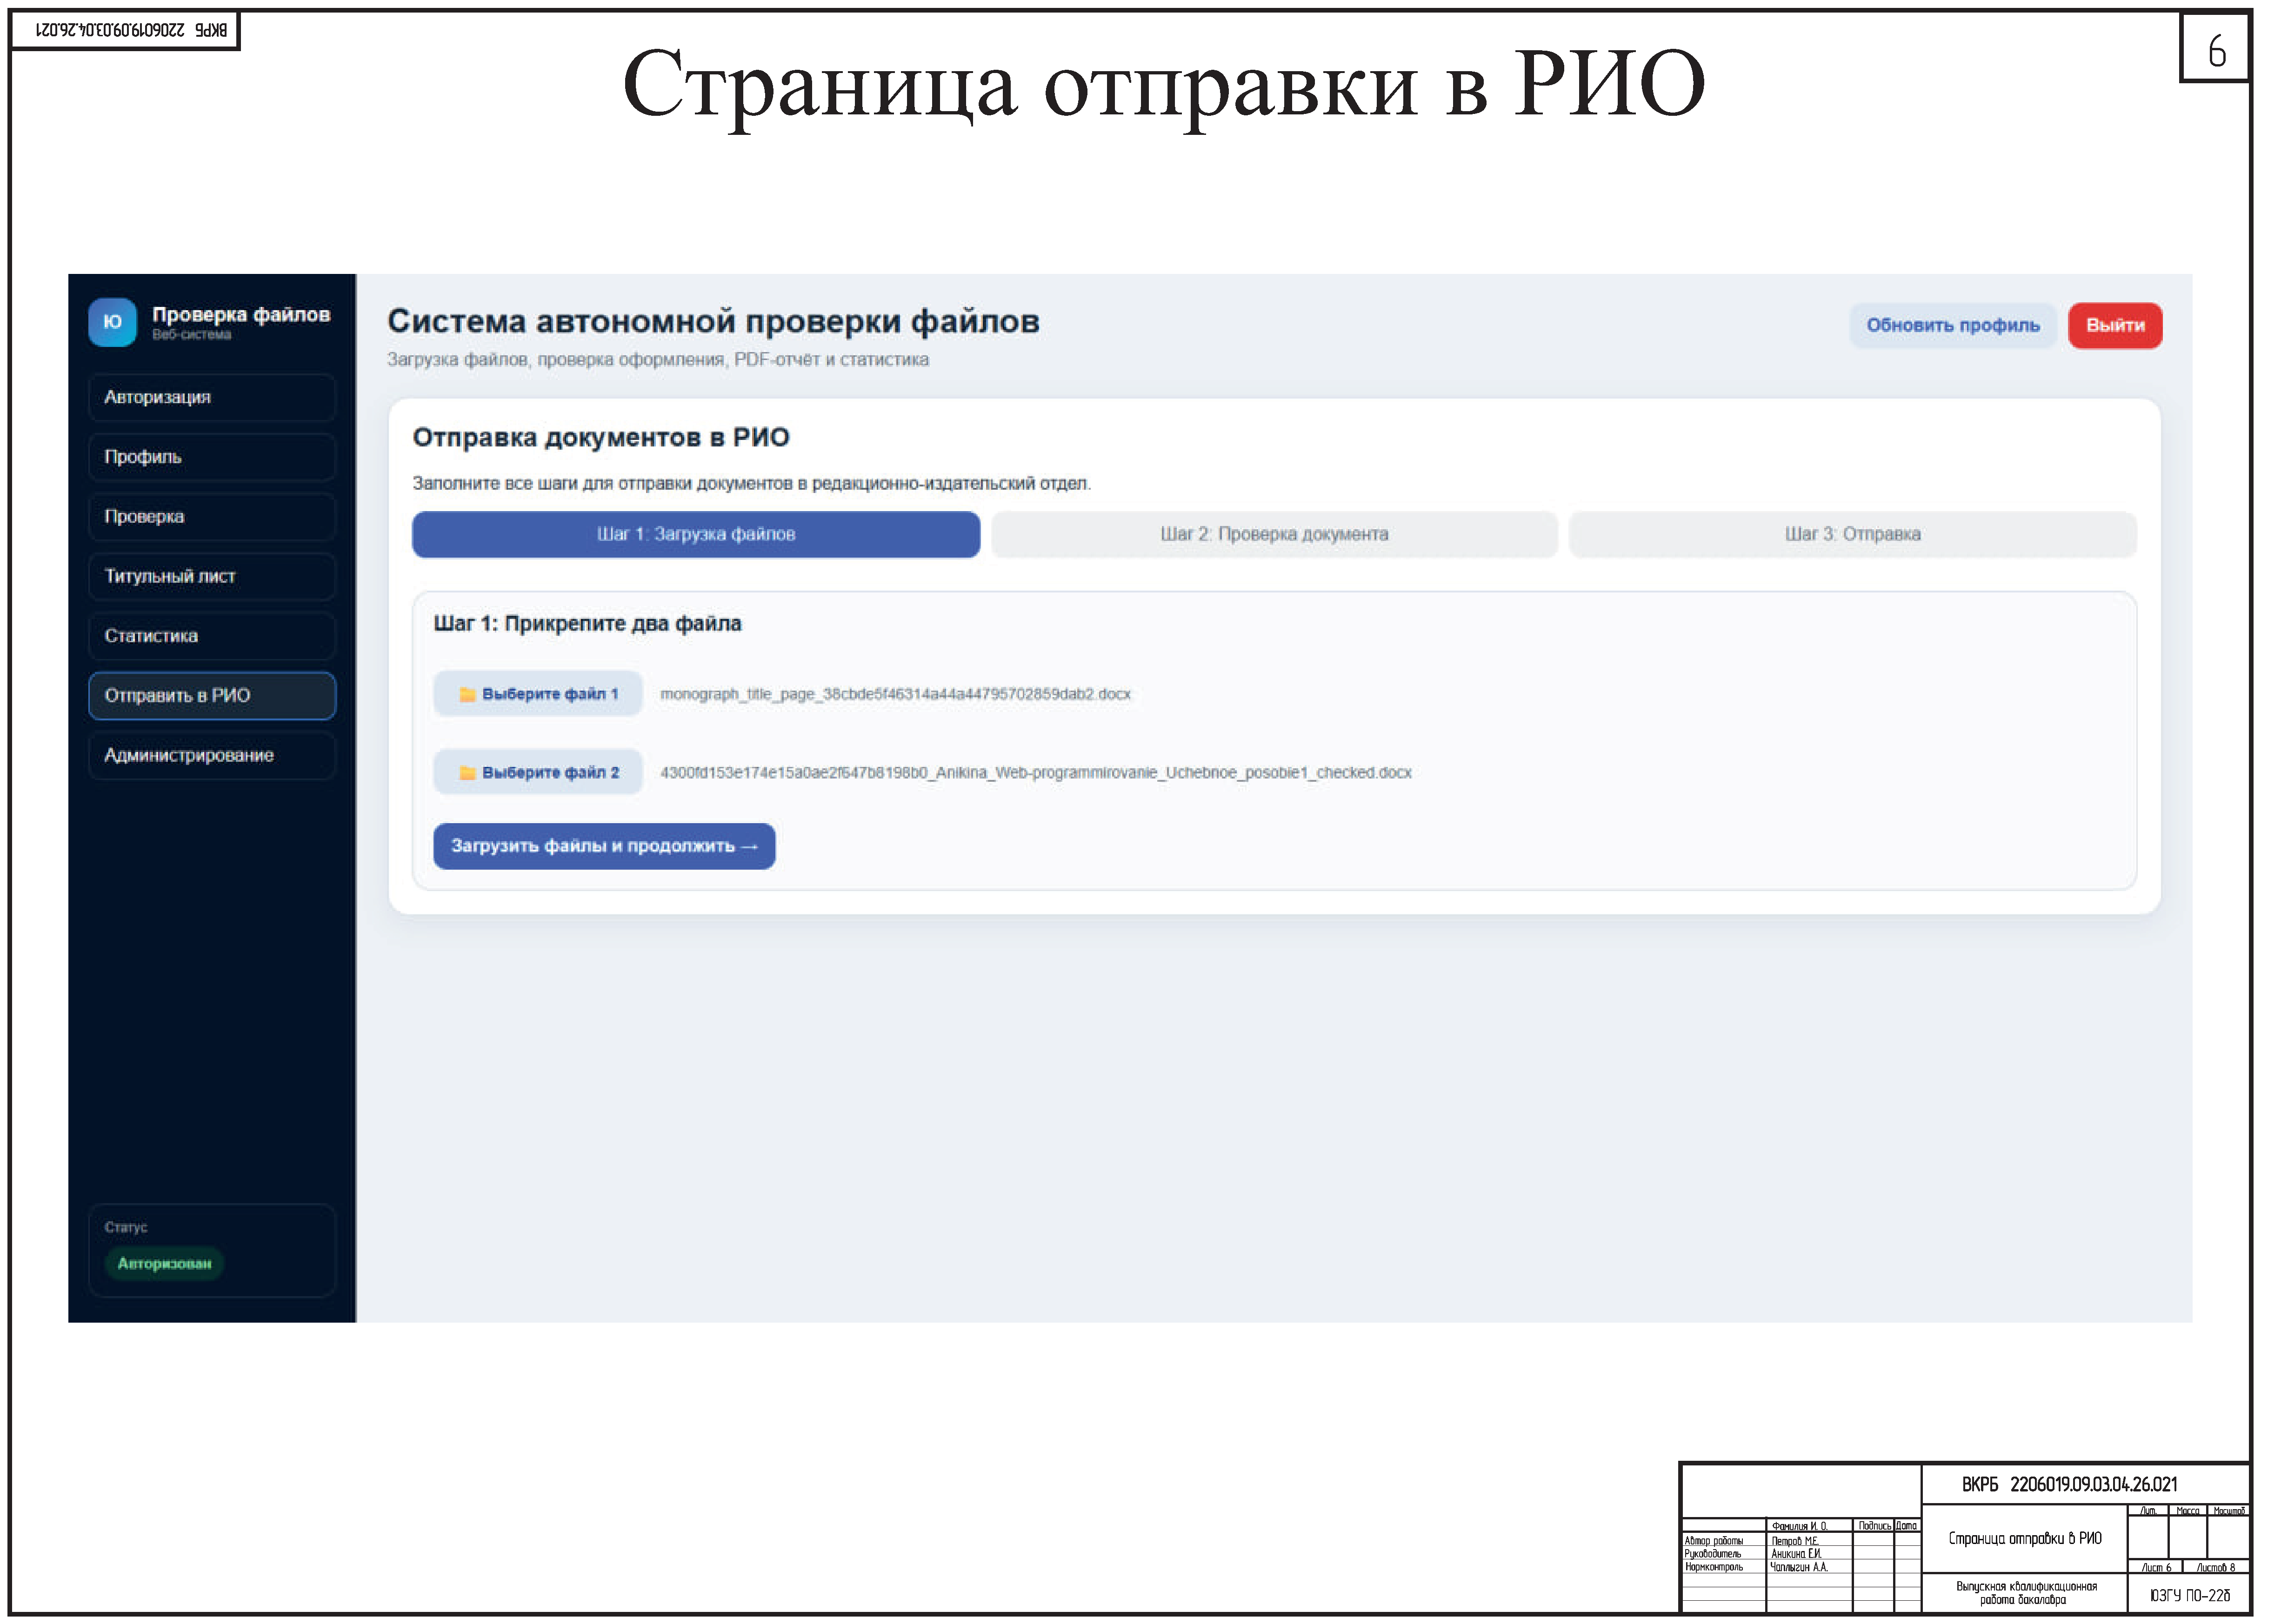
\includegraphics[width=0.82\linewidth]{Plakat6.eps}
		\заголовок{Страница отправки в РИО}
		\label{pl6:image}      
	\end{плакат}
	
	\begin{плакат}
		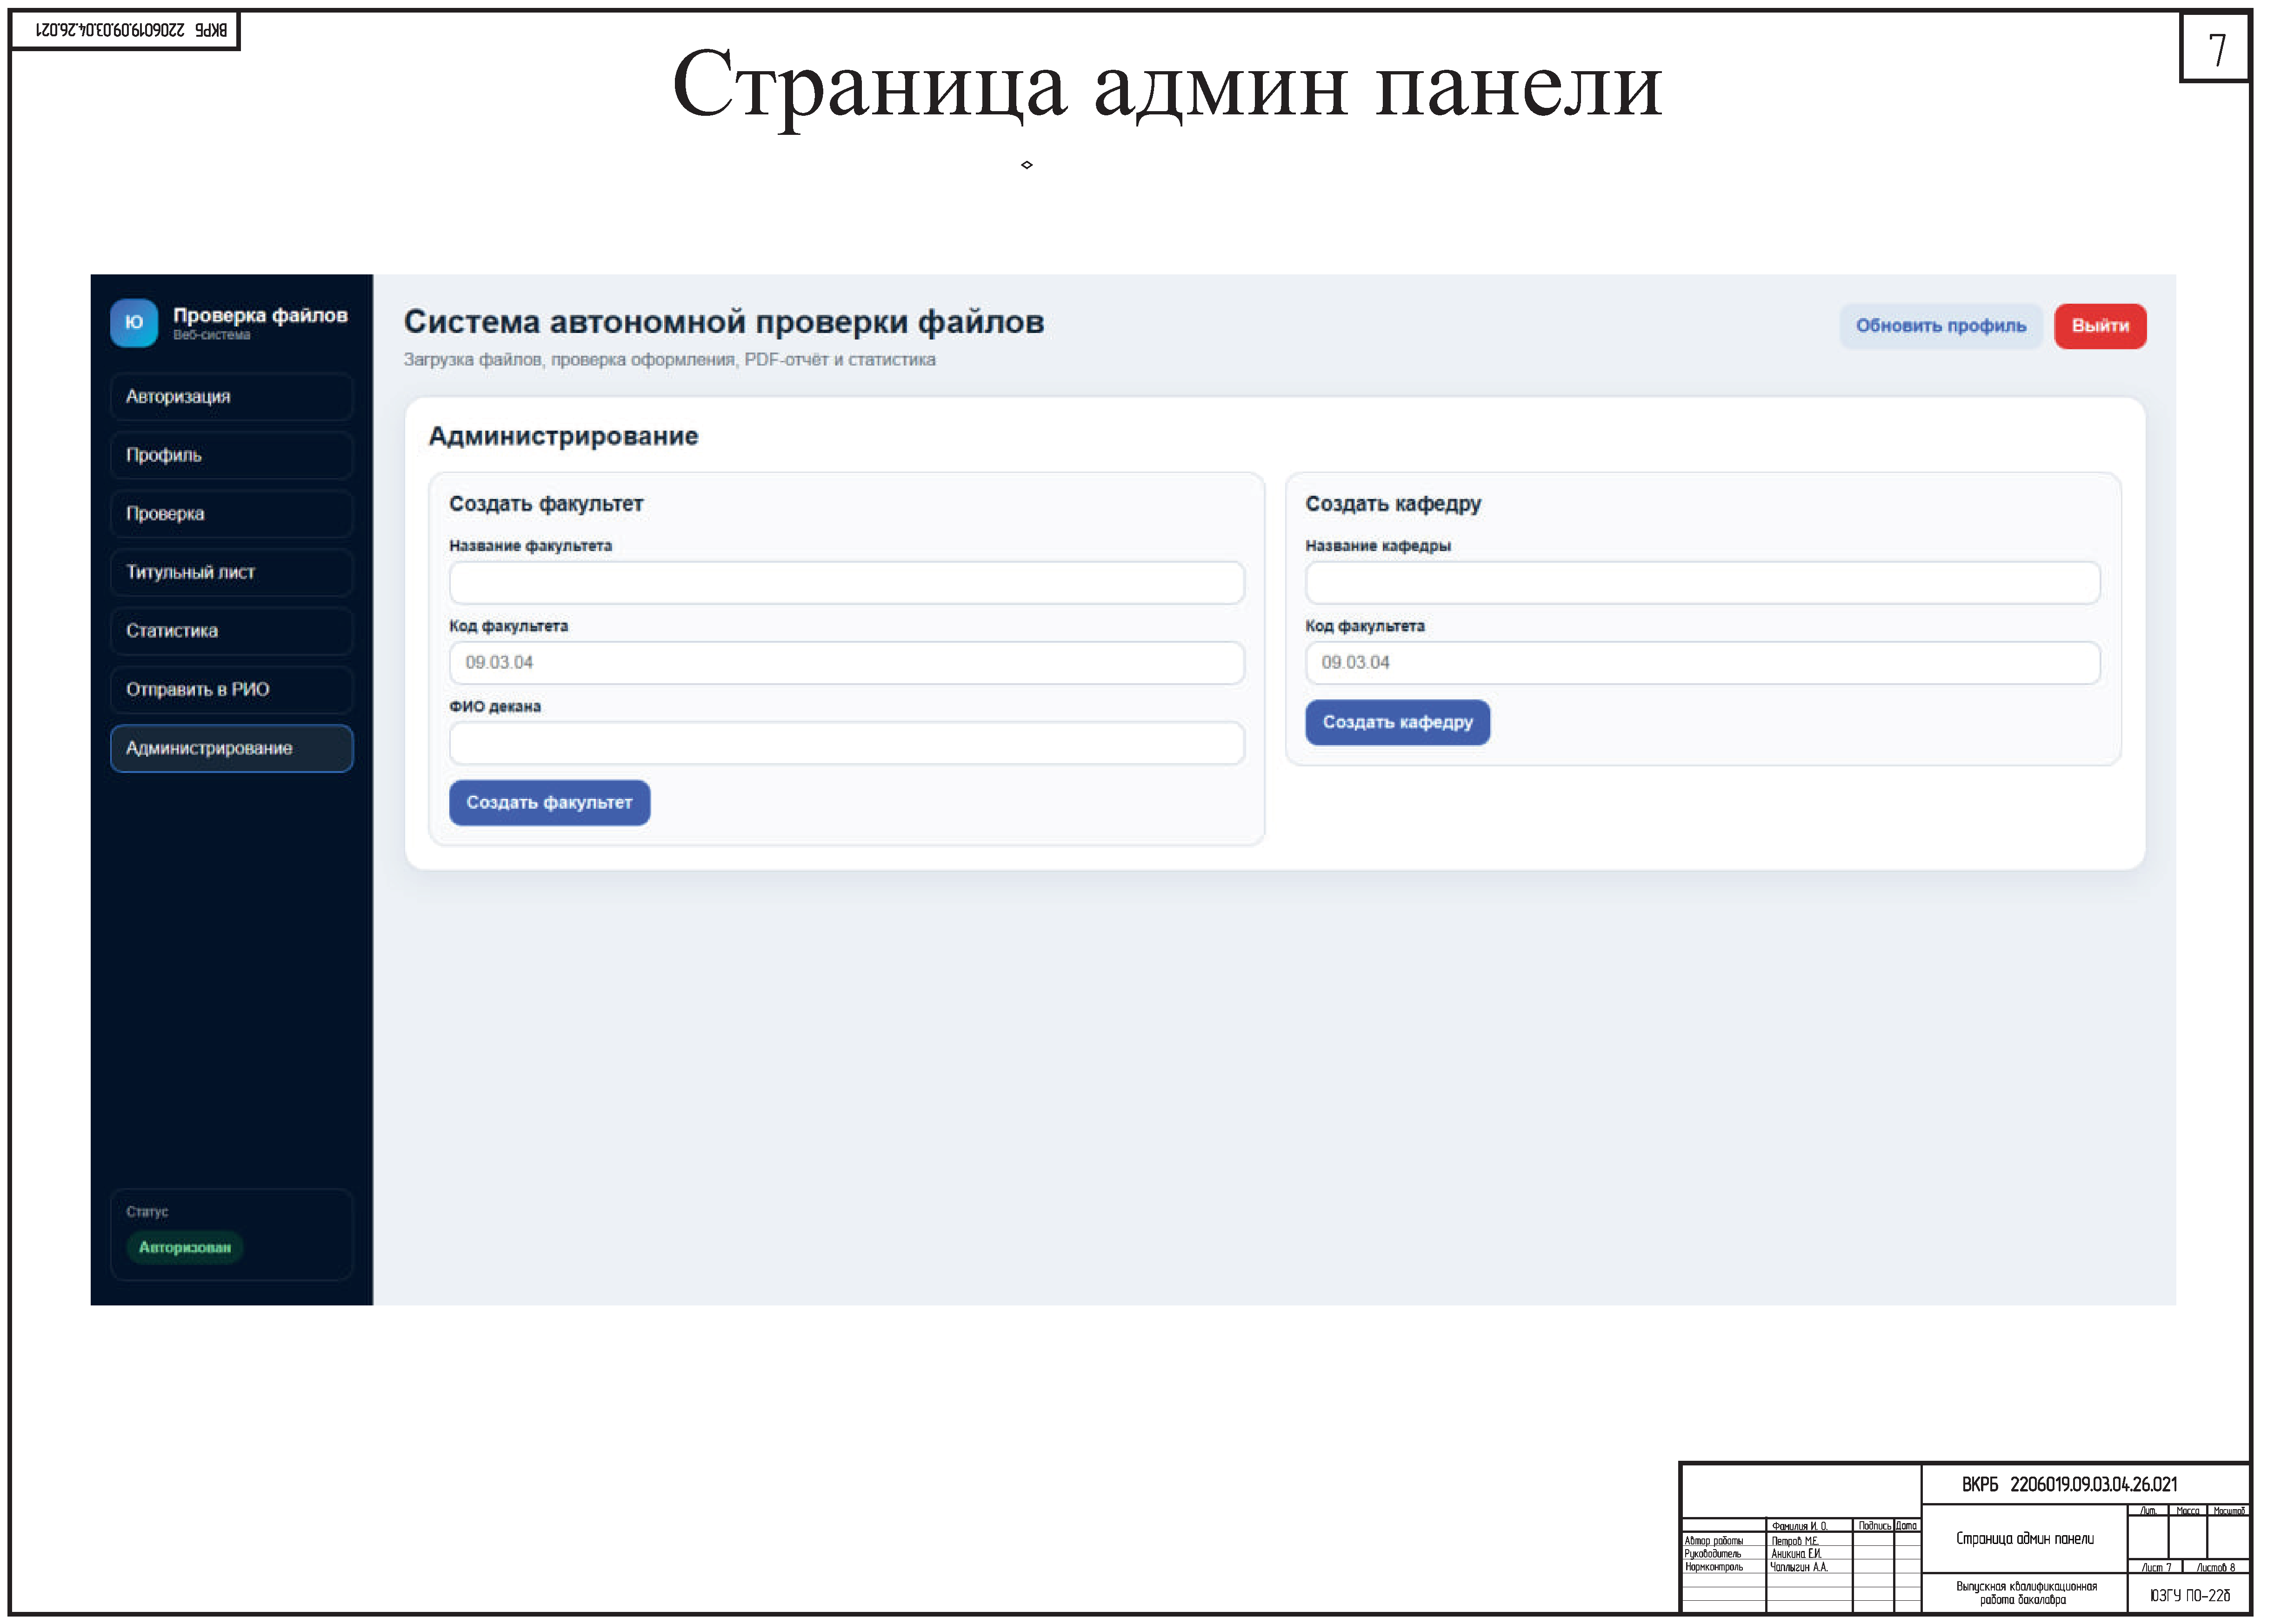
\includegraphics[width=0.82\linewidth]{Plakat7.eps}
		\заголовок{Страница админ панели}
		\label{pl7:image}      
	\end{плакат}
	
	\begin{плакат}
		
\includegraphics[width=0.82\linewidth]{Plakat8.eps}
		\заголовок{Заключение}
		\label{pl8:image}      
	\end{плакат}
	
\end{landscape}}\fi
\ifПрактика{}\else{\appendix{Фрагменты исходного кода программы}

main.py
\lstinputlisting[language=Python, frame=none]{main.py}

encoder.py
\lstinputlisting[language=Python, frame=none]{encoder.py}

save\_jpeg.py
\lstinputlisting[language=Python, frame=none]{save_jpeg.py}

color.py
\lstinputlisting[language=Python, frame=none]{color.py}

dct.py
\lstinputlisting[language=Python, frame=none]{dct.py}

quantization.py
\lstinputlisting[language=Python, frame=none]{quantization.py}

subsampling.py
\lstinputlisting[language=Python, frame=none]{subsampling.py}

ui.py
\lstinputlisting[language=Python, frame=none]{ui.py}

\ifВКР{
\newpage
\addcontentsline{toc}{section}{На отдельных листах (CD-RW в прикрепленном конверте)}
\begin{center}
\textbf{Место для диска}
\end{center}
}\fi
}\fi
\end{document}
